% Architectures examples: http://hal.archives-ouvertes.fr/docs/00/14/95/27/PDF/RR.pdf
\pdfminorversion=5 
\pdfobjcompresslevel=2
\documentclass{ltxdoc}
\usepackage[T1]{fontenc}
\usepackage[utf8]{inputenc}
\usepackage{amsmath}
\usepackage{lmodern}
\usepackage[ruled, lined,linesnumbered]{algorithm2e}

%% Use the tikz package and loading the library
%\usepackage{tikz}
%\usetikzlibrary{switching-architectures}

%% Loading only the package
\usepackage{sa-tikz}

\usepackage{calc}
\usepackage{imakeidx}

\usepackage[naturalnames]{hyperref}
    \hypersetup{%
        colorlinks=true,
        linkcolor=blue,
        filecolor=blue,
        urlcolor=blue,
        citecolor=blue,
        pdfborder=0 0 0,
    }

% dedicated commands:
\newcommand\Tikz{Ti\textit kZ}
\newcommand{\saTikZ}{S\textit{a}-\Tikz}

\def\pgfautoxrefs{1}
\input ./macros/pgfmanual-en-macros.tex

\makeatletter
\def\index@prologue{%
\section*{Index}\addcontentsline{toc}{section}{Index}
}
\makeatother

\usepackage{pgfmanual}

\pgfkeys{
    /pdflinks/search key prefixes in={/tikz/,/pgf/},
    /pdflinks/internal link prefix=pgfp,
    /pdflinks/codeexample links=true,
    /pdflinks/warnings=false,
    /pdflinks/show labels=false,
}
\makeindex
\newcommand{\version}{0.7}
\newcommand{\versiondate}{January 21, 2014}

\title{\saTikZ\footnote{This package has version number \textit{v}\version\ of \versiondate; it is released under and subject to the \href{http://www.latex-project.org/lppl/}{\LaTeX\ Project Public License (LPPL)}.}}
\author{Claudio Fiandrino \\ \small\href{mailto:claudio.fiandrino@gmail.com}{\texttt{claudio.fiandrino@gmail.com}}}
\date{\versiondate}

\begin{document}
\maketitle
\tableofcontents

\section*{Introduction}
\addcontentsline{toc}{section}{Introduction}
The \saTikZ\ library is a tool for drawing \emph{switching-architectures}. In particular, one of its aims, is to help students to verify the correctness of their exercises, but it could also help teachers in preparing lecture notes. The official webpage of the project is hosted on \href{http://cfiandra.github.io/Sa-TikZ/}{http://cfiandra.github.io/Sa-TikZ/} and a public  repository of the library can be found in \href{https://github.com/cfiandra/Sa-TikZ}{https://github.com/cfiandra/Sa-TikZ}.

The \saTikZ\ library can be loaded in a \LaTeX\ preamble by means of:
\begin{flushleft}
\verb|\usetikzlibrary{|\bgroup\color{red!75!black}\verb|switching-architectures|\egroup\verb|}|
\end{flushleft}
and in this case you should also load manually:
\begin{flushleft}
\verb|\usepackage{|\bgroup\color{red!75!black}\verb|tikz|\egroup\verb|}|
\end{flushleft}
or by means of:
\begin{flushleft}
\verb|\usepackage{|\bgroup\color{red!75!black}\verb|sa-tikz|\egroup\verb|}|
\end{flushleft}
In both cases the auxiliary \Tikz\ libraries \bgroup\color{red!75!black}\verb|calc|\egroup{}, \bgroup\color{red!75!black}\verb|decorations.pathreplacing|\egroup\ and \bgroup\color{red!75!black}\verb|positioning|\egroup\ are automatically loaded; in the latter case also the \Tikz\ package is loaded.

The version \textit{v}\version\ is compliant with \Tikz\ 3.0.0 and provides a way to draw Clos Networks Strictly-non-Blocking (snb) and Rearrangeable (rear), Benes Networks and Banyan Networks (in particular Omega\footnote{Implementation of Omega Networks by João Gabriel Reis.} and Flip Networks); moreover, the package provides the possibility to fully customize the aspect of the drawn network: the dimensions of module, their distance and the font used are some examples. Finally, \saTikZ\ let users to draw connections among the stages by accessing the single ports of the modules.

\section{Basic usage}
The simplest use of the package is to define a 
\begin{command}{{\node}}
    Basic command definition.
\end{command}
with one of the following options
\begin{key}{/tikz/clos snb}
    Option for drawing a Clos Network Strictly-non-Blocking.
\end{key}
\begin{key}{/tikz/clos rear}
    Option for drawing a Clos Network Rearrangeable.
\end{key}
\begin{key}{/tikz/benes}
    Option for drawing a Benes Network.
\end{key}
\begin{key}{/tikz/benes complete}
    Option for drawing a Benes Network with the lowest level of recursion.
\end{key}
\begin{key}{/tikz/banyan omega}
    Option for drawing an Banyan-Omega Network.
\end{key}
\begin{key}{/tikz/banyan flip}
    Option for drawing an Banyan-Omega Network with inverse shuffle exchange (Flip).
\end{key}
inside a |tikzpicture| environment:
\begin{environment}{{tikzpicture}\opt{\oarg{options}}}
\end{environment}

\subsection{Examples of Clos Networks}

The following example shows a Rearrangeable Clos Network.

\begin{codeexample}[]
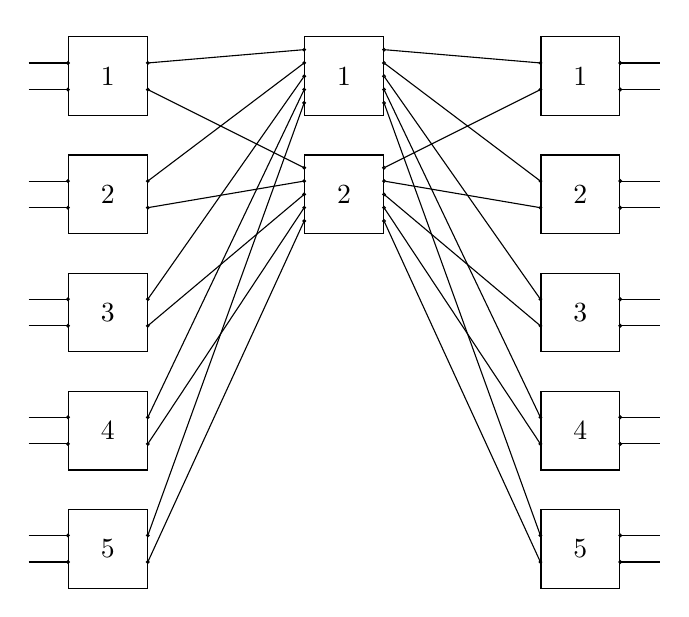
\begin{tikzpicture}
    \node[clos rear] {};
\end{tikzpicture}
\end{codeexample}

The following example shows a Strictly-non-Blocking Clos Network.

\begin{codeexample}[]
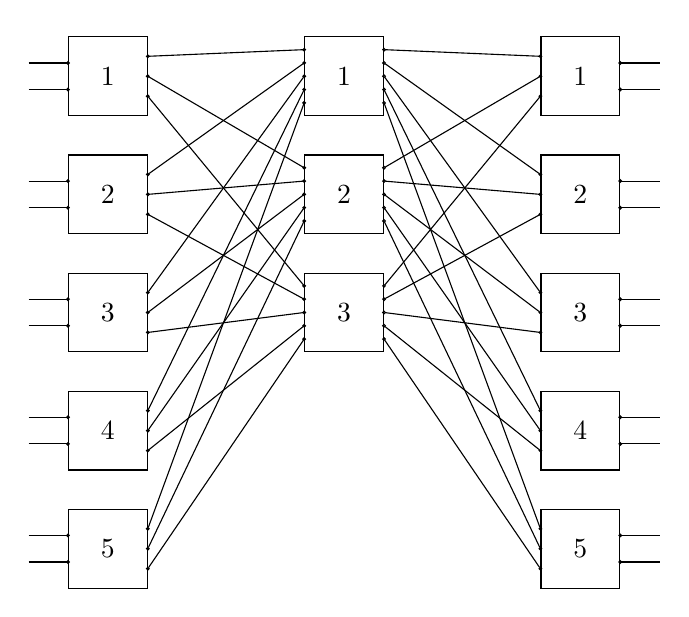
\begin{tikzpicture}
    \node[clos snb] {};
\end{tikzpicture}
\end{codeexample}

Notice from the examples that the library is able to compute \textit{automatically} the constraints defining a Clos Network to be Strictly-non-Blocking or Rearrangeable. The network drawn is characterized by:
\begin{itemize}
\item the first stage with:
\begin{itemize}
\item a number of modules equal to 5;
\item each one with two input ports;
\end{itemize}
\item the last stage with:
\begin{itemize}
\item a number of modules equal to 5;
\item each one with two output ports.
\end{itemize}
\end{itemize}
Each module of the network is numbered according to the stage it belongs to.

\subsection{Examples of Benes Networks}

The simplest example of a Benes Network:
\begin{codeexample}[]
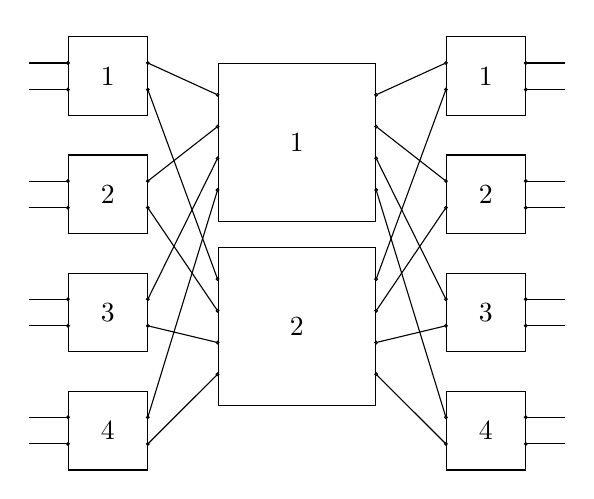
\begin{tikzpicture}
    \node[benes] {};
\end{tikzpicture}
\end{codeexample}
is a Benes Network in which there are 8 input and output ports. To draw a Benes Network in which all modules are visible, the key |benes complete| should be used rather than the |benes| key. An example:

\begin{codeexample}[]
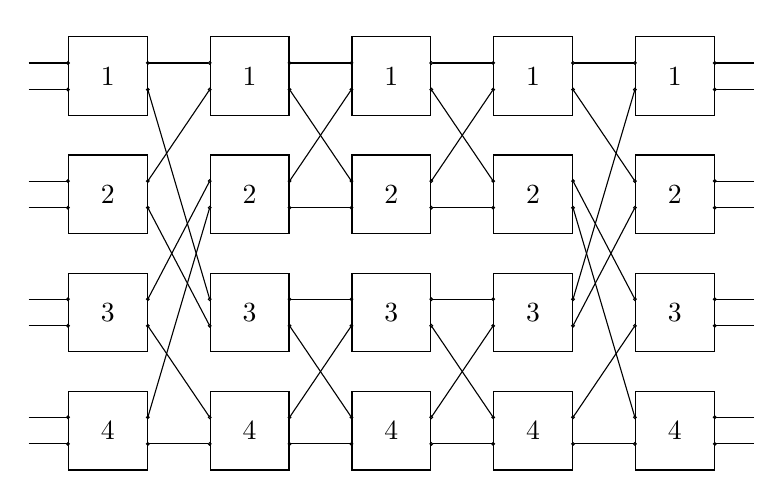
\begin{tikzpicture}
    \node[benes complete] {};
\end{tikzpicture}
\end{codeexample}

The algorithm in which the internal connections of the |benes complete| networks are drawn is explained in detail in the appendix \ref{sec:benesconnalg}.

\subsection{Examples of Banyan Networks}

The following examples show the two Banyan Network architectures that \saTikZ\ can draw.

\bgroup
\tikzset{every node/.append style={scale=0.9,transform shape}}
\begin{codeexample}[]
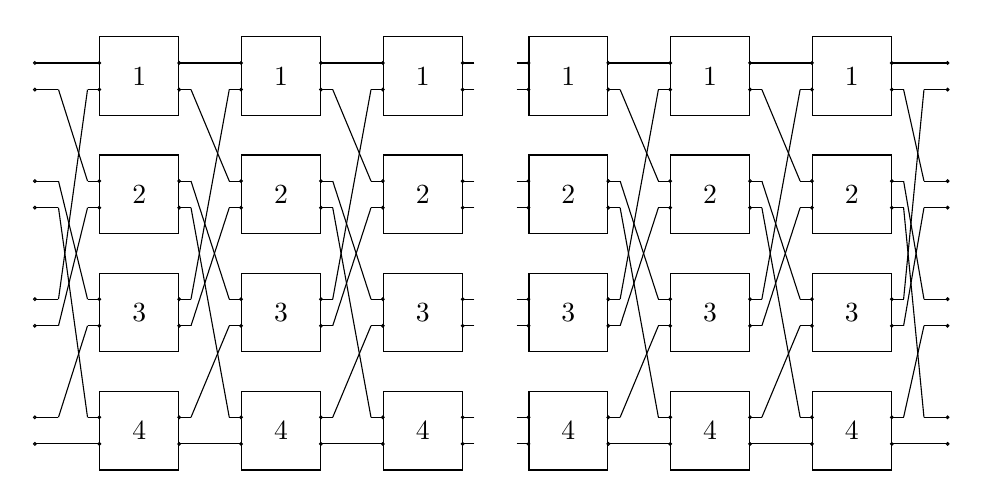
\begin{tikzpicture}
    % Omega Network on the left
    \node[banyan omega] {};
    \begin{scope}[xshift=7.25cm]
    	   % Flip network on the right
       \node[banyan flip]{};
    \end{scope}
\end{tikzpicture}
\end{codeexample}
\tikzset{every node/.append style={scale=1,transform shape}}
\egroup

\section{The options}
\subsection{Designing choices}
This subsection provides a detailed analysis of the options and parameters that can be used to draw Clos, Benes and Omega Networks. In particular:
\begin{itemize}
\item Clos Networks are analysed in \ref{subsubsec:clos};
\item Benes Networks are analysed in \ref{subsubsec:benes};
\item Banyan Networks are analysed in \ref{subsubsec:banyan}.
\end{itemize}
Each subsection presents the keys' definitions and simple examples to help the reader. 

\subsubsection{Clos Networks}
\label{subsubsec:clos}
The two first important design parameters are the total number of input ports of the first stage and the total number of output ports of the last stage. These two parameters could be customized by means of:

\begin{key}{/tikz/N=\marg{value} (initially 10)}
    This is the number of total input ports in the first stage.
\end{key}

\begin{key}{/tikz/M=\marg{value} (initially 10)}
    This is the number of total output ports in the last stage.
\end{key}

Usually, a second important design parameter is the number of modules present in the first and last stage. \saTikZ\ defines:

\begin{key}{/tikz/r1=\marg{value} (initially 5)}
    This is the number of modules in the first stage.
\end{key}

\begin{key}{/tikz/r3=\marg{value} (initially 5)}
    This is the number of modules in the last stage.
\end{key}

The two design parameters provide the number of ports of each module:
\[m_1=\dfrac{N}{r_1} \hspace*{2cm} m_3=\dfrac{M}{r_3} \]

Some examples considering |N|=9, |r1|=3, |M|=9 and |r3|=3.
\begin{codeexample}[]
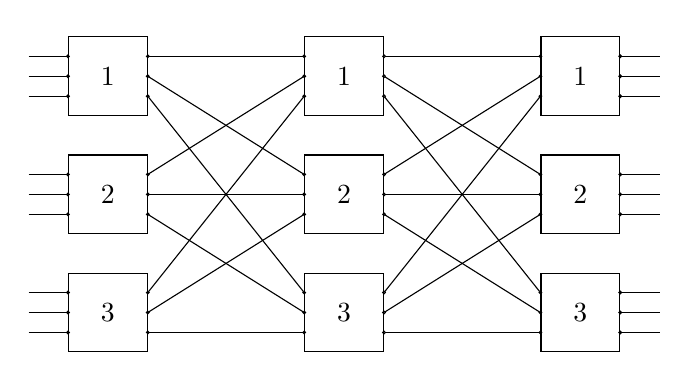
\begin{tikzpicture}
    \node[N=9,r1=3,M=9,r3=3,clos rear] {};
\end{tikzpicture}
\end{codeexample}

\begin{codeexample}[]
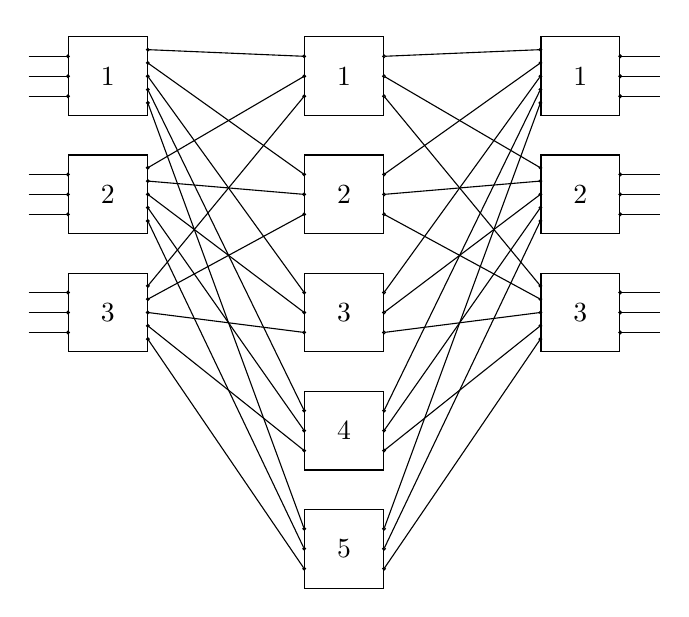
\begin{tikzpicture}
    \node[N=9,r1=3,M=9,r3=3,clos snb] {};
\end{tikzpicture}
\end{codeexample}

Notice a very important thing: when the keys are set within the \cs{node}, the type of the architecture should be loaded \emph{after} all the design parameters; if this constraint is not respected, you will end up with an architecture which has default values. For example:

\begin{codeexample}[]
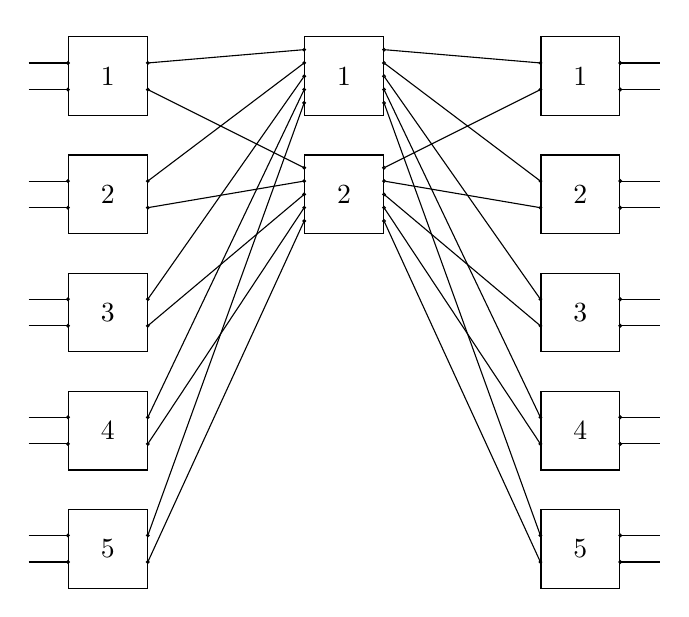
\begin{tikzpicture}
    \node[clos rear,N=9,r1=3,M=9,r3=3] {};
\end{tikzpicture}
\end{codeexample}

\subsubsection{Benes Networks}
\label{subsubsec:benes}
Benes Networks are Clos Rearrangeable Networks composed of $2 \times 2$ modules. Hence, as design choice, it just possible to select the number of input/output ports:

\begin{key}{/tikz/P=\marg{value} (initially 8)}
    This is the number of total input/output ports in the first/third stage.
\end{key}

Notice that |P| could assume values
\[P=2^p \qquad p=2,3,4,\ldots\]
and the user is responsible to correctly set this parameter.

For low values of $p$ there are no problems in visualizing the network, but as $p$ increases, the user should take care of the modules' dimension and the modules' separation (vertical and horizontal): these parameters could be customized as explained in the subsection \ref{subsec:customization}. Actually, for |benes complete| networks, the number of $p$ is crucial: when it is above 7, namely the network is bigger than $128\times 128$, PGF can not properly work due to internal limitations.

Notice that, for |P|=4 the |benes| network and the |benes complete| network are indistinguishable:
\begin{codeexample}[]
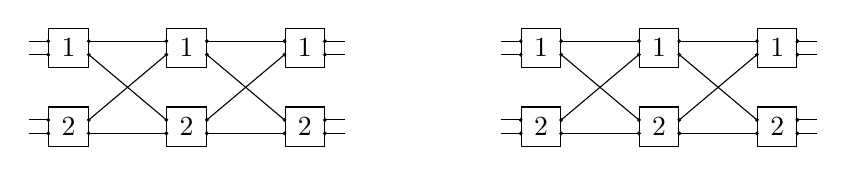
\begin{tikzpicture}
\tikzset{module size=0.5cm,
 pin length factor=0.5,
 module ysep=1}
 \node[P=4,benes] {};
 \begin{scope}[xshift=6cm]
     \node[module xsep=2.5,P=4,benes complete]{};
 \end{scope}
\end{tikzpicture}
\end{codeexample}

Here is an example of Benes Network with |P|=16:
\begin{codeexample}[]
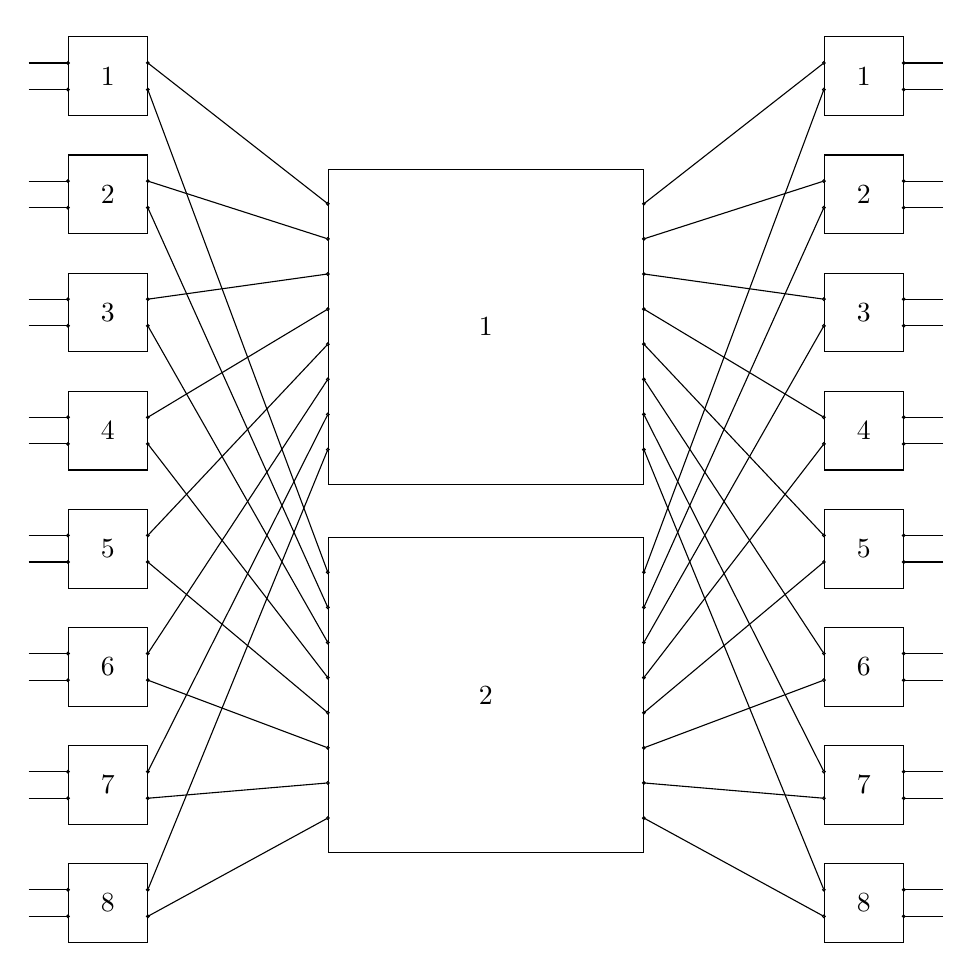
\begin{tikzpicture}
    \node[P=16,benes] {};
\end{tikzpicture}
\end{codeexample}

It holds the same concept afore-mentioned for Clos Networks: set the parameter |P| before declaring the \cs{node} to be a Benes Network.

\subsubsection{Banyan Networks}
\label{subsubsec:banyan}
Banyan Networks are architectures based on Benes Networks: they have particular interconnections properties. As well as Benes Networks, only the number of inputs and outputs ports can be selected and it is |P|.

\saTikZ is able to represent Omega and Flip Banyan Networks. Omega networks are based on João Gabriel Reis' implementation.  An example of $4\times 4$ |banyan omega| network:
\begin{codeexample}[]
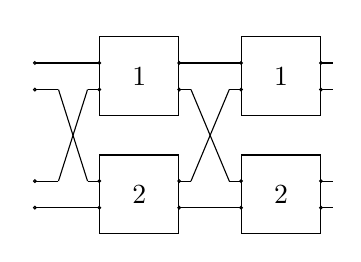
\begin{tikzpicture}
    \node[P=4,banyan omega] {};
\end{tikzpicture}
\end{codeexample}

An example of $4\times 4$ |banyan flip| network:
\begin{codeexample}[]
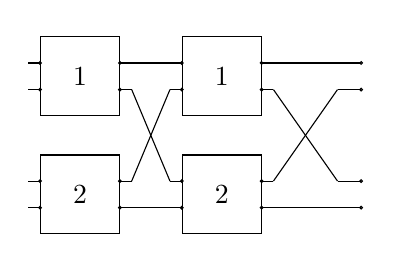
\begin{tikzpicture}
    \node[P=4,banyan flip] {};
\end{tikzpicture}
\end{codeexample}

\subsection{Output customization}
\label{subsec:customization}
This subsection presents the keys devoted to customize the networks' aspect.

\begin{key}{/tikz/module size=\marg{value} (initially 1cm)}
    This option allows to set the module dimension.
\end{key}

\begin{key}{/tikz/module ysep=\marg{value} (initially 1.5)}
    This option allows to set the vertical module distance factor.
\end{key}

\begin{key}{/tikz/module xsep=\marg{value} (initially 3)}
    This option allows to set the horizontal module distance factor.
\end{key}

\begin{key}{/tikz/module label opacity=\marg{value} (initially 1)}
    This option allows to mask the module label when the \meta{value} is set to 0.
\end{key}

\begin{key}{/tikz/pin length factor=\marg{value} (initially 1)}
    This option allows to reduce/increase the length of the pins drawn in input/output. Use a \meta{value} [0,1] to reduce the length or, viceversa, a \meta{value} greater than 1 to increase the length.
\end{key}

\begin{key}{/tikz/module font=\marg{font commands} (default \cs{normalfont})}
    This option sets the font used for module labels. The \meta{font commands} that could be used are those ones related to the font size (i.e. \cs{Large}) and font shape (i.e \cs{itshape}).
\end{key}

\begin{key}{/tikz/connections disabled=\mchoice{true,false} (default false)}
	This option, not active by default |connections disabled/.default=false|, allows to remove the connections between the stages when it is set to \opt{true}. Beware: this option is valid only for |clos snb|, |clos rear|, |benes| and |benes complete| networks, but it does not holds for the architectures explained in section \ref{sec:dida}.
\end{key}

The following example shows a Rearrangeable Clos Network with some custom options. Notice that the |module label opacity| should be given as parameter of the desired network.

\begin{codeexample}[]
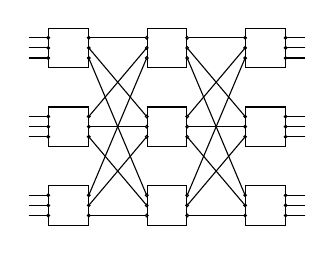
\begin{tikzpicture}[N=9,r1=3,M=9,r3=3]
    \node[module size=0.5cm,pin length factor=0.5,
        module ysep=1, module xsep=1.25,
        clos rear={module label opacity=0}] {};
\end{tikzpicture}
\end{codeexample}

The options could be also introduced with the standard \Tikz\ syntax:
\begin{command}{{\tikzset}\marg{options}}
    Command that process the various \meta{options}: they should be provided separated by commas.
\end{command}

Therefore, the previous example can be modified into:
\begin{codeexample}[]
\tikzset{module size=0.5cm,pin length factor=0.5,
         module ysep=1, module xsep=1.25,}
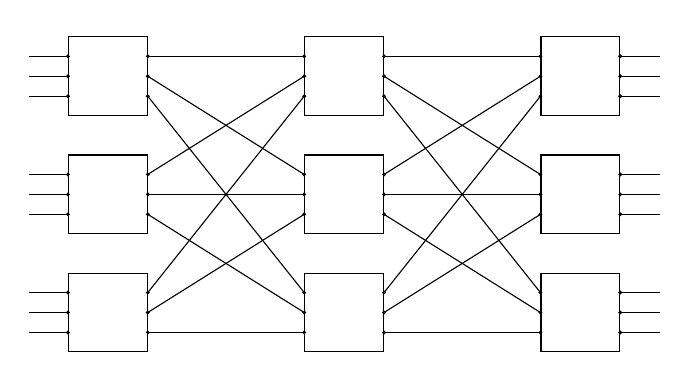
\begin{tikzpicture}[N=9,r1=3,M=9,r3=3]
    \node[clos rear={module label opacity=0}] {};
\end{tikzpicture}
\end{codeexample}

It is also possible to declare \opt{styles} to set some options for later use: this helps to keep the code clean especially when the same options are re-used several times; an example:
\begin{codeexample}[code only]
\tikzset{module size definition/.style={
  module size=0.75cm,
  pin length factor=0.75,
  module xsep=2,
  module ysep=2,
  }
}
\tikzset{module size definition, 
 P=16,
}
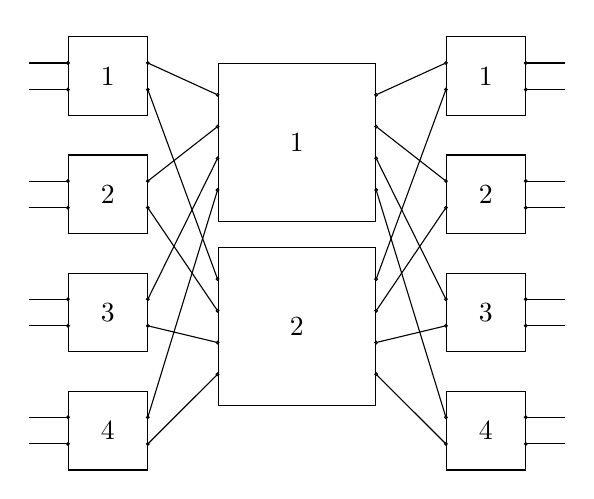
\begin{tikzpicture}
    \node[benes] {};
\end{tikzpicture}
\end{codeexample}

Here is a Benes Network $4 \times 4$ which presents an extremely large font size for the module labels and its interconnection paths are disabled:
\begin{codeexample}[]
\tikzset{my style/.style={
  module size=0.75cm,
  pin length factor=0.75,
  module xsep=2,
  }
}
\tikzset{my style, P=4, 
 module font=\huge\slshape, 
 connections disabled=true
}
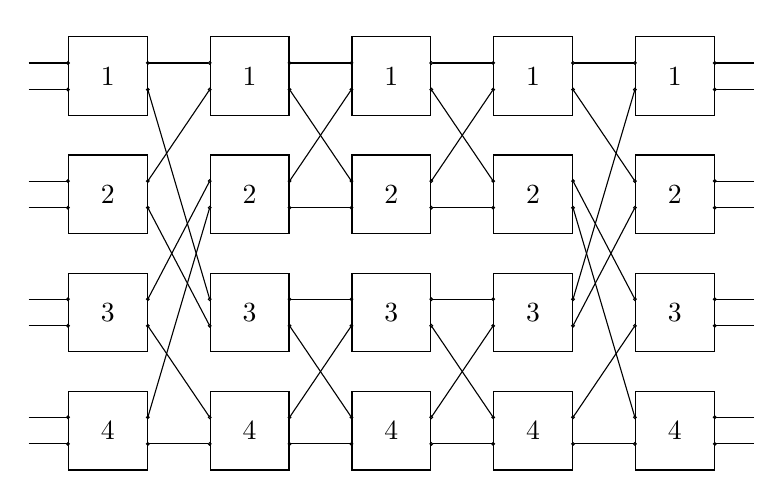
\begin{tikzpicture}
    \node[benes complete] {};
\end{tikzpicture}
\end{codeexample}

Consider the following $16 \times 16$ Omega Network:
\begin{codeexample}[]
\tikzset{module size=0.6cm,pin length factor=0.6,
         module ysep=0.65, module xsep=3.5,}
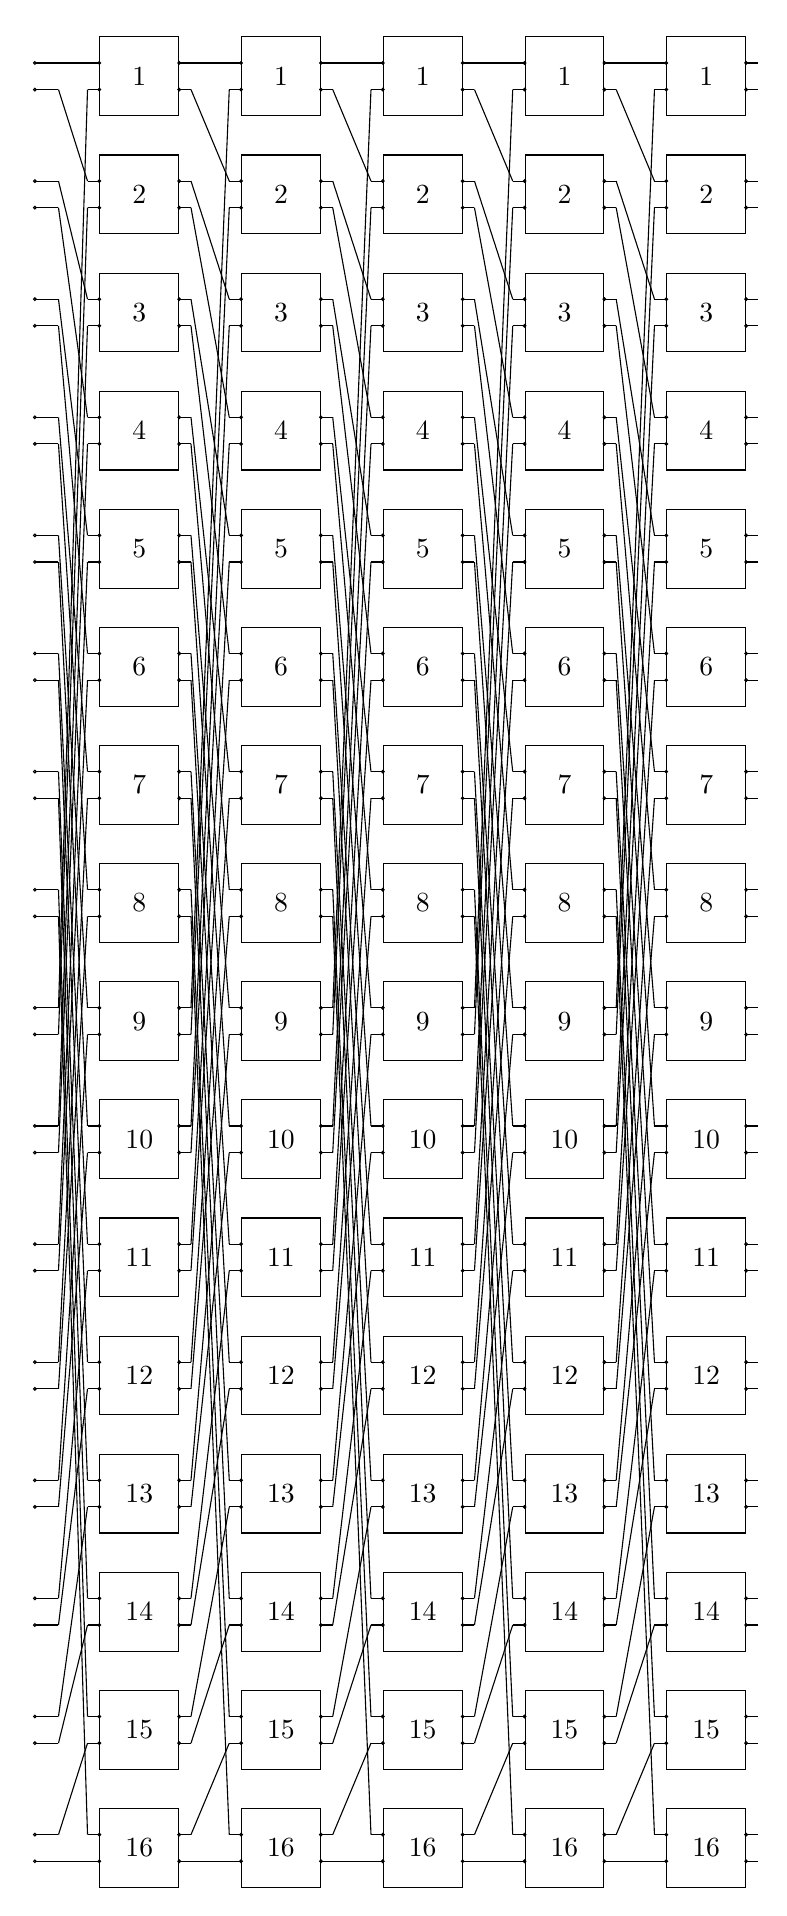
\begin{tikzpicture}[P=32]
    \node[banyan omega] {};
\end{tikzpicture}
\end{codeexample}

\pagebreak

An example of Benes Network $32 \times 32$:
\begin{codeexample}[]
\tikzset{module size=0.6cm,pin length factor=0.6,
         module ysep=0.9, module xsep=1.7,}
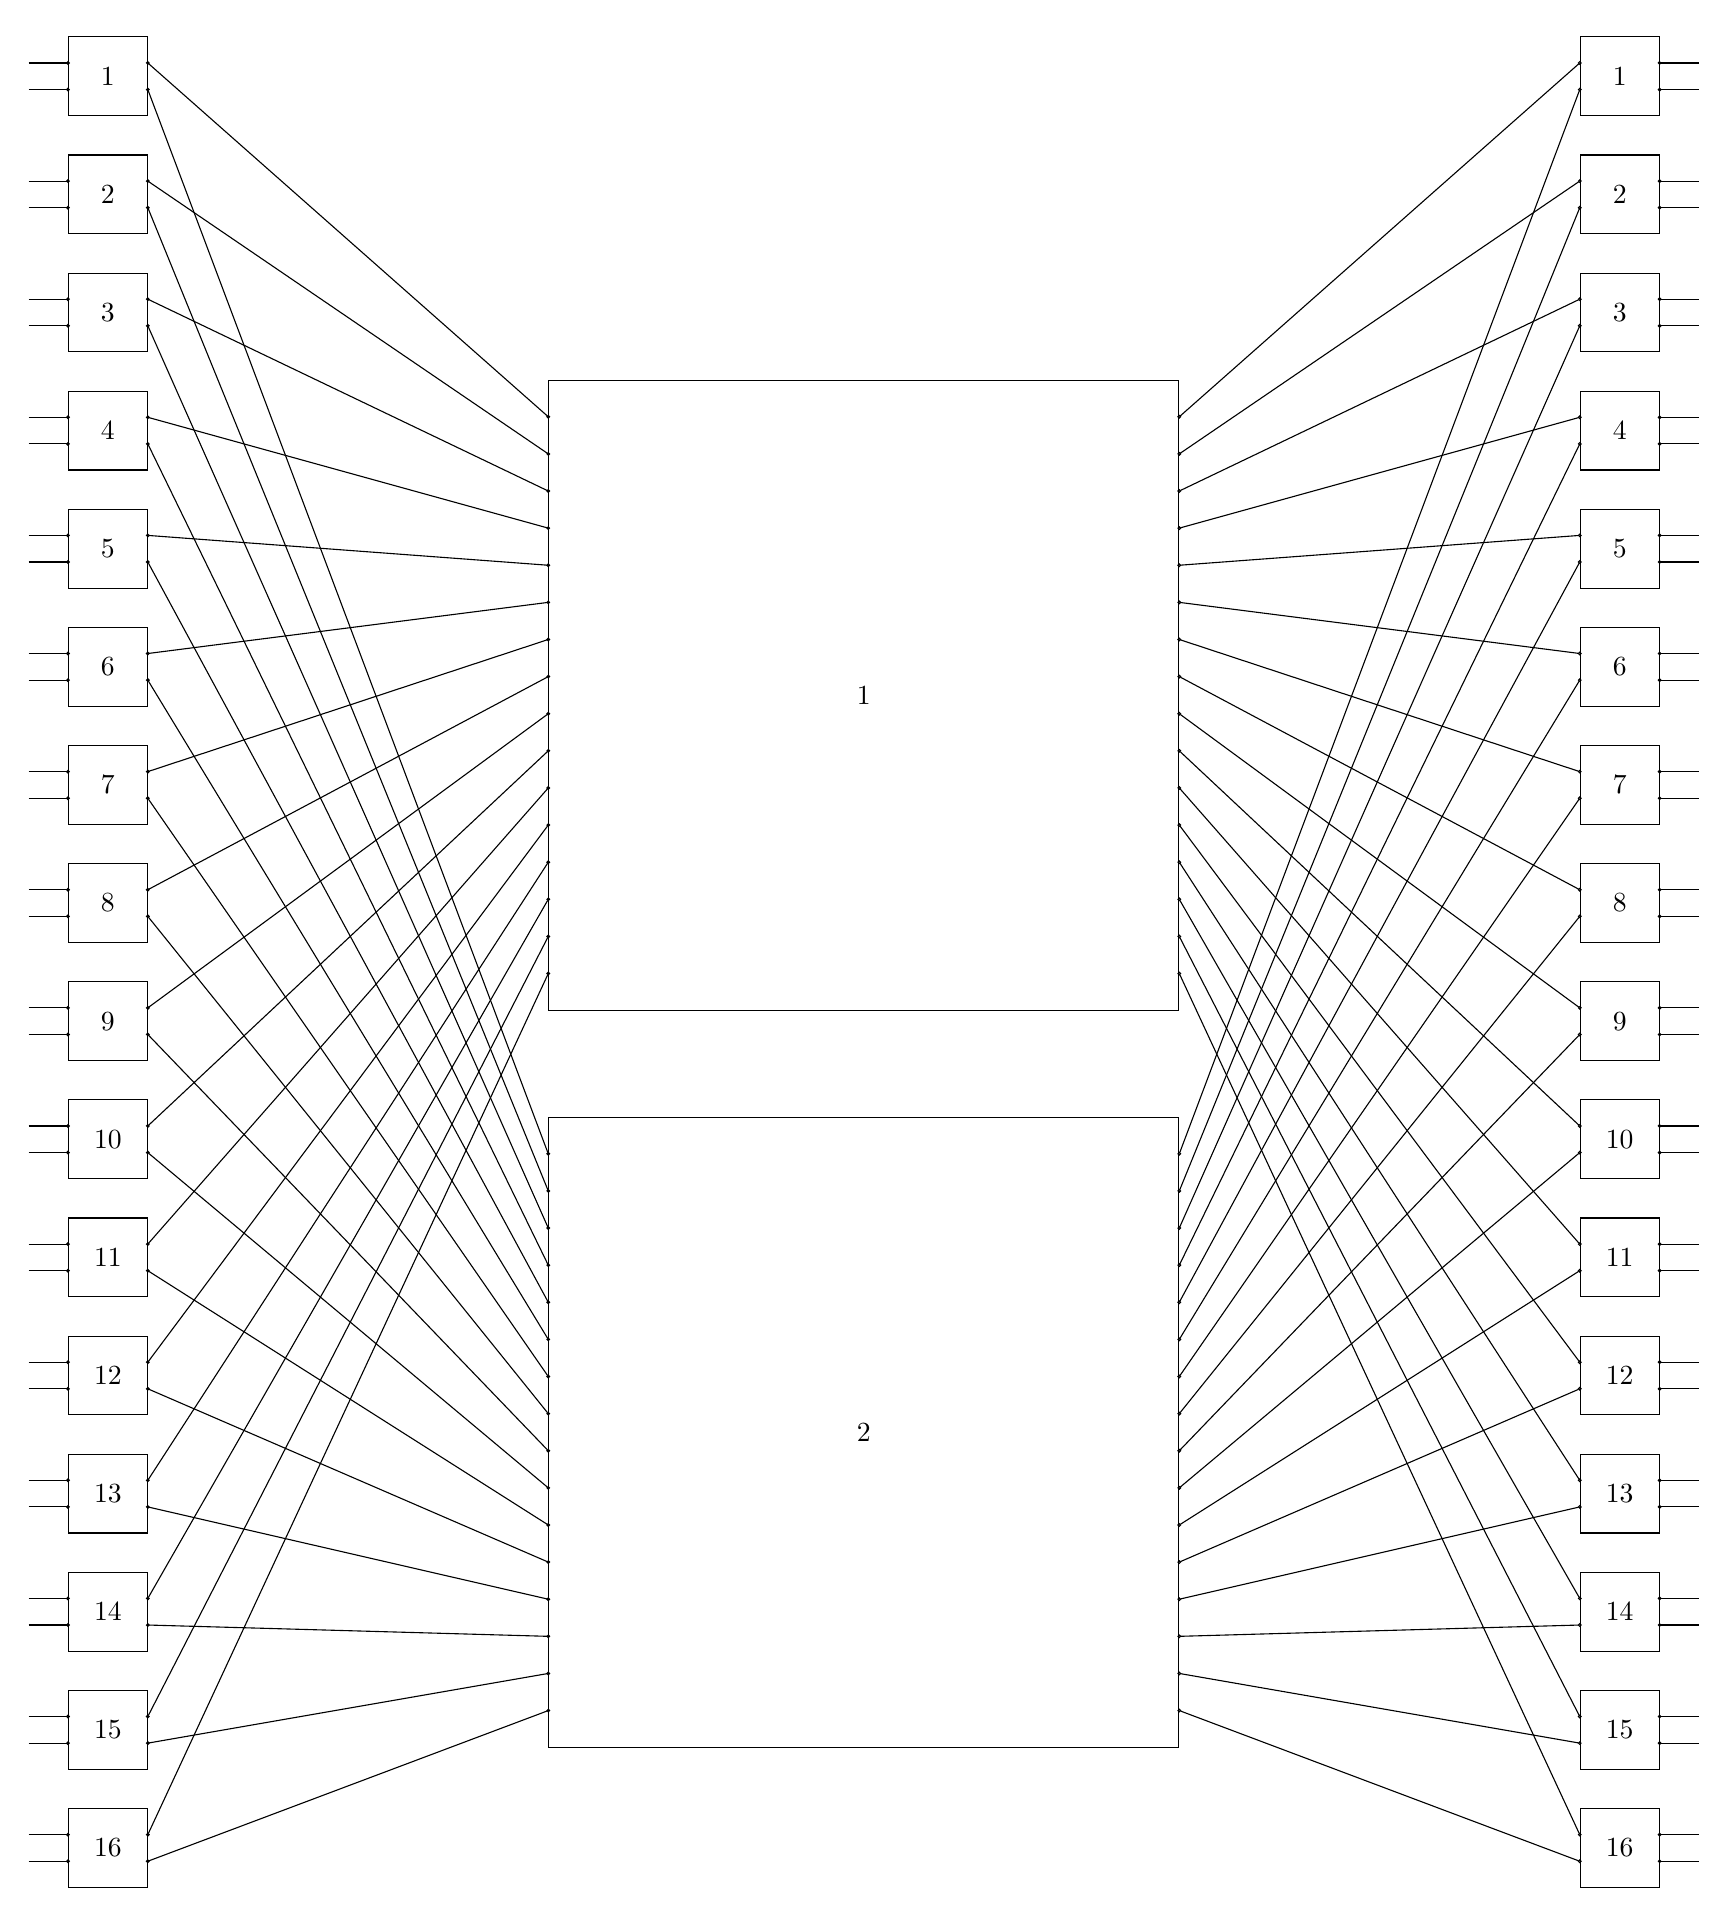
\begin{tikzpicture}[P=32]
    \node[benes] {};
\end{tikzpicture}
\end{codeexample}
\pagebreak

and its complete form:
\begin{codeexample}[]
\tikzset{module size=0.6cm,pin length factor=0.6,
         module ysep=1, module xsep=2.275}
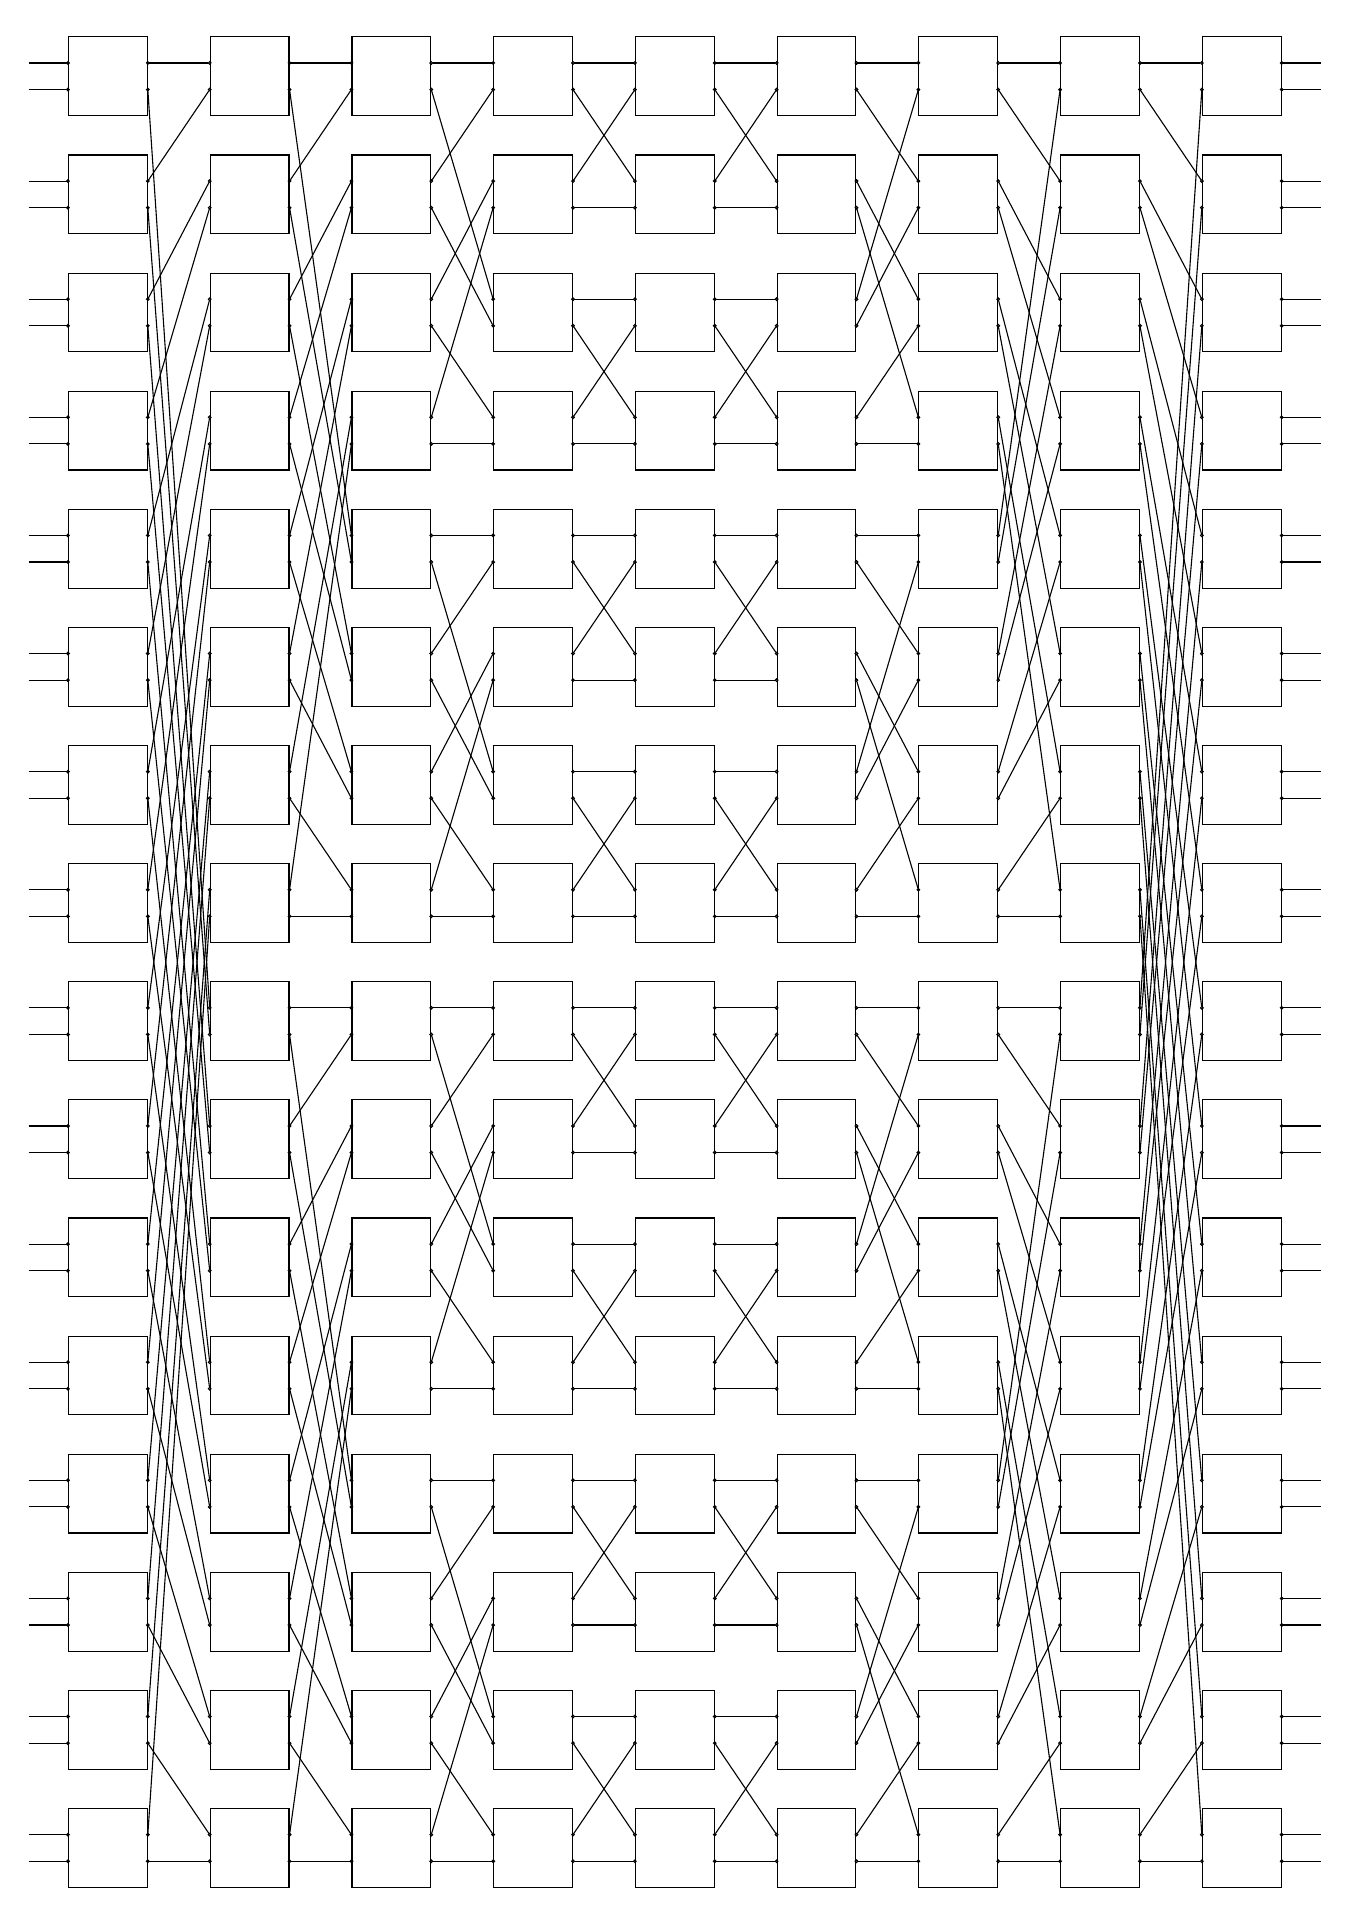
\begin{tikzpicture}[P=32]
    \node[benes complete={module label opacity=0}] {};
\end{tikzpicture}
\end{codeexample}


\section{Advanced usage}
This section presents some more advanced examples. More in detail, it is described how to add elements to the basic architecture; the elements can be:
\begin{itemize}
\item labels for the input and output ports;
\item paths interconnecting input and output ports.
\end{itemize}

\subsection{Identifying front input/output ports}
In this subsection it is shown how to reference the front input and output ports for the first and last stage. Each front input port could be accessed by means of:
\begin{flushleft}
\verb|r1-|\bgroup\color{red!75!black}\verb|module number|\egroup\verb|-|\bgroup\color{red!75!black}\verb|front input|\egroup\verb|-|\bgroup\color{red!75!black}\verb|port number|\egroup; example: \verb|r1-1-front input-1|;
\end{flushleft}
Each front output port could be accessed by means of:
\begin{flushleft}
\verb|r3-|\bgroup\color{red!75!black}\verb|module number|\egroup\verb|-|\bgroup\color{red!75!black}\verb|front output|\egroup\verb|-|\bgroup\color{red!75!black}\verb|port number|\egroup; example: \verb|r3-1-front output-1|;
\end{flushleft}
Noticed that the first stage is always 1, but the last stage may be different from 3 in case the |benes complete| network is drawn. Errors will occur in case the last stage number is not correct and the user is responsible for the correct setting.

A simple example with a Rearrangeable Clos network of 4 input and output ports; the first stage and the last one have both 2 modules.

\begin{codeexample}[]
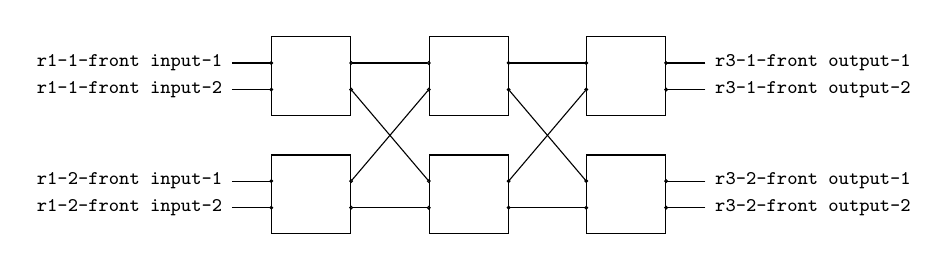
\begin{tikzpicture}[module xsep=2]
  \node[N=4,r1=2,M=4,r3=2,clos rear={module label opacity=0}] {};
  \foreach \name 
    in {r1-1-front input-1,r1-1-front input-2,
        r1-2-front input-1,r1-2-front input-2}
    \node[left] at (\name) {\scriptsize{\texttt{\name}}};
  \foreach \name 
    in {r3-1-front output-1,r3-1-front output-2,
        r3-2-front output-1,r3-2-front output-2}
    \node[right] at (\name) {\scriptsize{\texttt{\name}}};
\end{tikzpicture}
\end{codeexample}

The following is a Strictly-non-Blocking Clos network of 9 input and output ports in which the first and last stage have 3 modules each one.

\begin{codeexample}[]
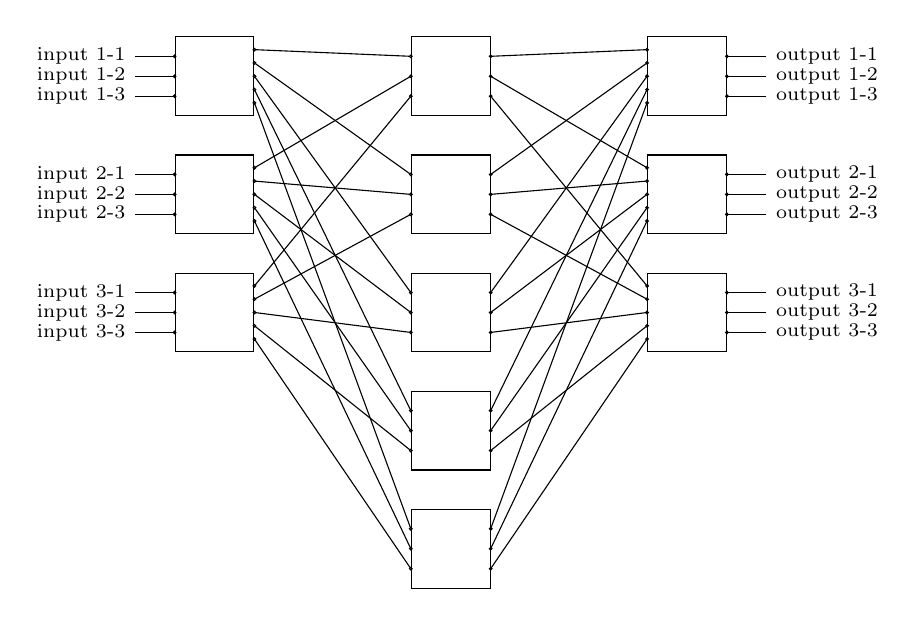
\begin{tikzpicture}
    \node[N=9,r1=3,M=9,r3=3,clos snb={module label opacity=0}] {};

	\foreach \startmodule in {1,...,3}{
		\foreach \port in {1,...,3}
				 \node[left] at (r1-\startmodule-front input-\port)
				 {\scriptsize{input \startmodule-\port}}; 
	}
	\foreach \startmodule in {1,...,3}{
		\foreach \port in {1,...,3}
				 \node[right] at (r3-\startmodule-front output-\port)
				 {\scriptsize{output \startmodule-\port}}; 
	}    
\end{tikzpicture}
\end{codeexample}

The same applies also for Benes Networks:
\begin{codeexample}[]
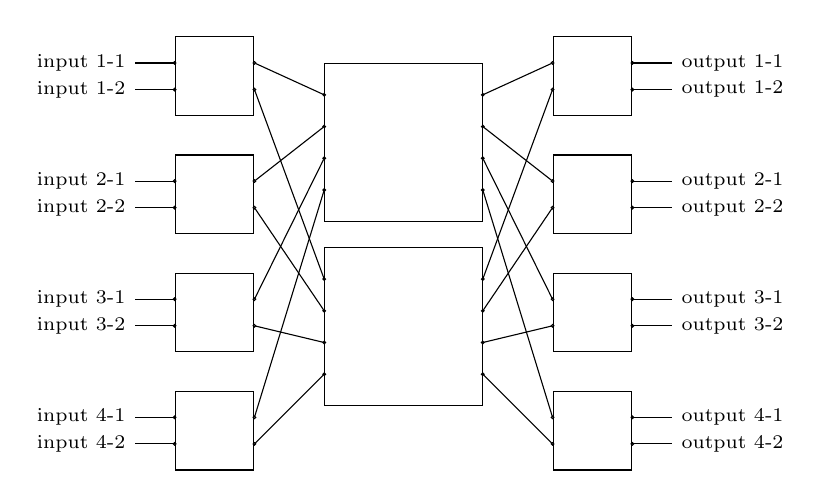
\begin{tikzpicture}
    \node[benes={module label opacity=0}] {};

	\foreach \startmodule in {1,...,4}{
		\foreach \port in {1,...,2}
				 \node[left] at (r1-\startmodule-front input-\port)
				 {\scriptsize{input \startmodule-\port}}; 
	}
	\foreach \startmodule in {1,...,4}{
		\foreach \port in {1,...,2}
				 \node[right] at (r3-\startmodule-front output-\port)
				 {\scriptsize{output \startmodule-\port}}; 
	}    
\end{tikzpicture}
\end{codeexample}
and to the correspondent complete form:
\begin{codeexample}[]
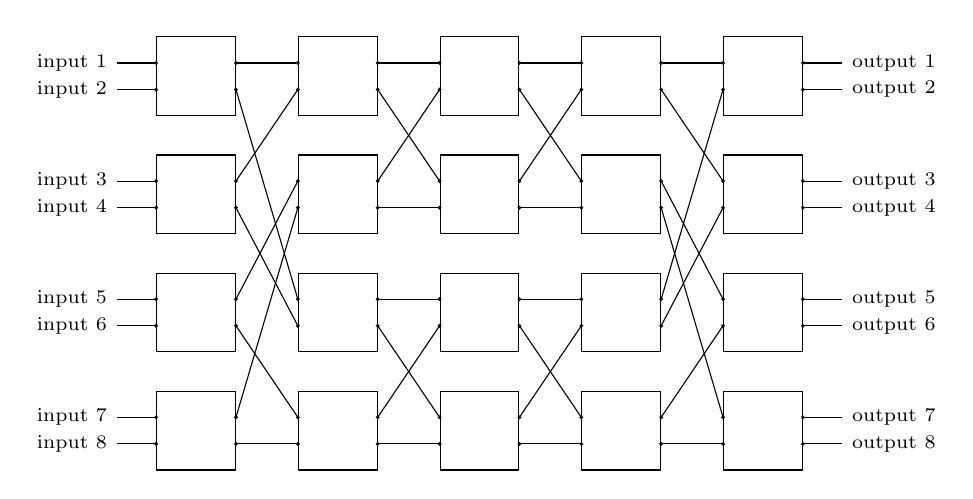
\begin{tikzpicture}
	\node[benes complete={module label opacity=0}] {};
	\newcounter{port}
	\setcounter{port}{0}
	\foreach \startmodule in {1,...,4}{
		\foreach \port in {1,...,2}
				\stepcounter{port}
				 \node[left] at (r1-\startmodule-front input-\port)
				 {\scriptsize{input \theport}}; 
	}
	\setcounter{port}{0}
	\foreach \startmodule in {1,...,4}{
		\foreach \port in {1,...,2}
				\stepcounter{port}
				 \node[right] at (r5-\startmodule-front output-\port)
				 {\scriptsize{output \theport}}; 
	}    
\end{tikzpicture}
\end{codeexample}
Notice that in this case to access the \verb|front output| ports, the stage number correct is 5 and not 3 as usual.

Ti\textit{k}Z has very useful \verb|bin(|$x$\verb|)| function: it converts $x$ (it is assumed to be a 10 base integer) into its binary representation. Exploiting this function for Omega or Flip Networks is very convenient. An example of Omega Network:
\begin{codeexample}[]
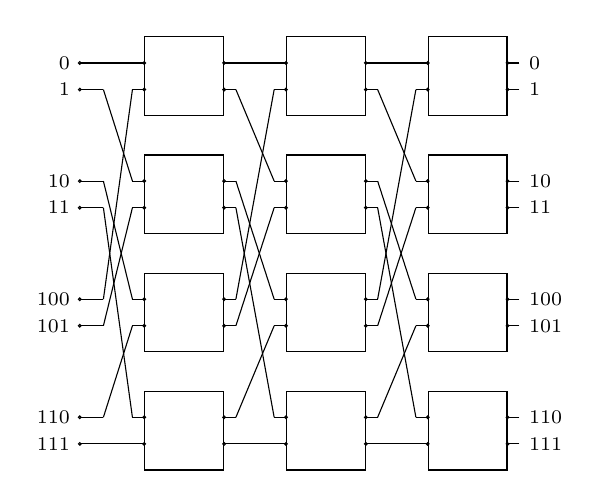
\begin{tikzpicture}
	\node[banyan omega={module label opacity=0}] {};
	\newcounter{porta}
	\setcounter{porta}{0}
	\foreach \module in {1,...,4}{
		\foreach \port in {1,...,2}{
				\stepcounter{porta}
				\pgfmathbin{\theporta-1}% get the binary value of the counter
				\node[left] at (r0-\module-front input-\port)
				 {\scriptsize{\pgfmathresult}}; 
				\node[right] at (r3-\module-front output-\port)
				 {\scriptsize{\pgfmathresult}};
		}
	}   
\end{tikzpicture}
\end{codeexample}

An example of Flip Network:
\begin{codeexample}[]
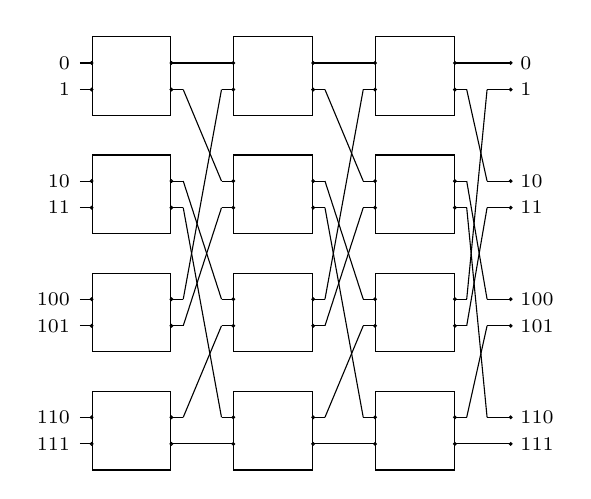
\begin{tikzpicture}
	\node[banyan flip={module label opacity=0}] {};
	\newcounter{portb}
	\setcounter{portb}{0}
	\foreach \module in {1,...,4}{
		\foreach \port in {1,...,2}{
				\stepcounter{portb}
				\pgfmathbin{\theportb-1}
				\node[left] at (r0-\module-front input-\port)
				 {\scriptsize{\pgfmathresult}}; 
				\node[right] at (r3-\module-front output-\port)
				 {\scriptsize{\pgfmathresult}};
		}
	}   
\end{tikzpicture}
\end{codeexample}
Notice that for Banyan Networks the first module is characterized by number 0 and not 1.

\subsection{Identifying input/output ports per module}

It is also possible to access, for each module of each stage, its input and output ports. The syntax is similar to the one used for the front input and output ports; each input port could be accessed by means of:
\begin{flushleft}
\verb|r|\bgroup\color{red!75!black}\verb|stage number|\egroup\verb|-|\bgroup\color{red!75!black}\verb|module number|\egroup\verb|-|\bgroup\color{red!75!black}\verb|input|\egroup\verb|-|\bgroup\color{red!75!black}\verb|port number|\egroup; example: \verb|r1-1-input-1|;
\end{flushleft}
Each output port could be accessed by means of:
\begin{flushleft}
\verb|r|\bgroup\color{red!75!black}\verb|stage number|\egroup\verb|-|\bgroup\color{red!75!black}\verb|module number|\egroup\verb|-|\bgroup\color{red!75!black}\verb|front output|\egroup\verb|-|\bgroup\color{red!75!black}\verb|port number|\egroup; example: \verb|r2-1-output-1|;
\end{flushleft}
This allows to derive connections from the first stage to the last stage. Here is an example. 

\begin{codeexample}[]
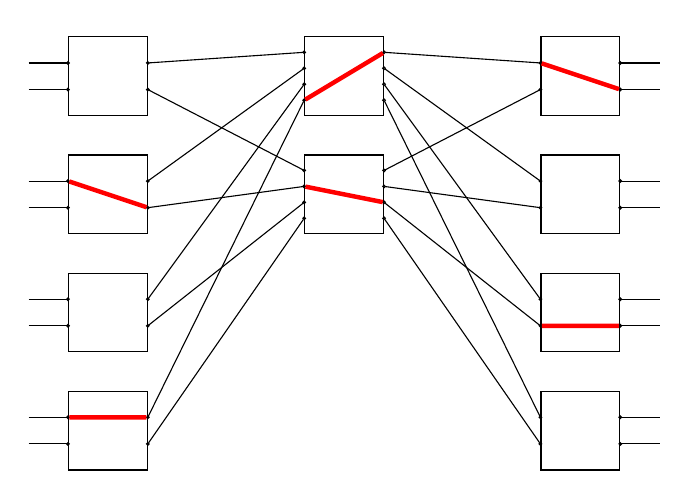
\begin{tikzpicture}
    \node[N=8,r1=4,M=8,r3=4,clos rear={module label opacity=0}] {};
    \draw[red,ultra thick](r1-2-input-1)--(r1-2-output-2) 
    	(r2-2-input-2)--(r2-2-output-3)
    	(r3-3-input-2)--(r3-3-output-2);
   	\draw[red,ultra thick](r1-4-input-1)--(r1-4-output-1) 
    	(r2-1-input-4)--(r2-1-output-1)
    	(r3-1-input-1)--(r3-1-output-2);
\end{tikzpicture}
\end{codeexample}
Similarly, an example in a Benes Network:
\begin{codeexample}[]
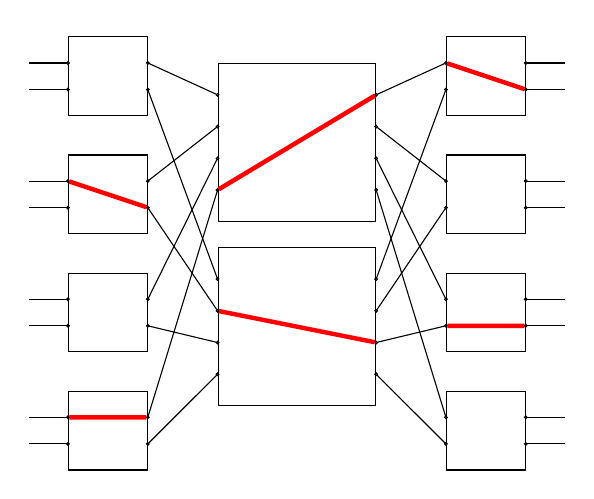
\begin{tikzpicture}
    \node[benes={module label opacity=0}] {};
    \draw[red,ultra thick](r1-2-input-1)--(r1-2-output-2) 
    	(r2-2-input-2)--(r2-2-output-3)
    	(r3-3-input-2)--(r3-3-output-2);
   	\draw[red,ultra thick](r1-4-input-1)--(r1-4-output-1) 
    	(r2-1-input-4)--(r2-1-output-1)
    	(r3-1-input-1)--(r3-1-output-2);
\end{tikzpicture}
\end{codeexample}
and in its complete form:
\begin{codeexample}[]
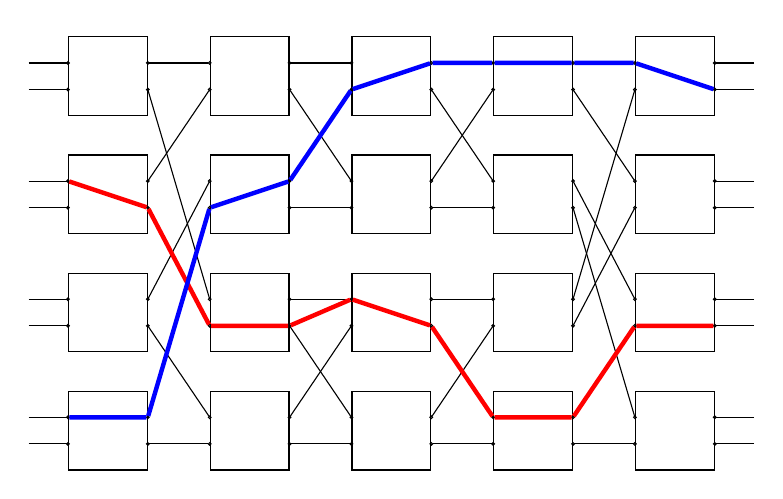
\begin{tikzpicture}
    \node[benes complete={module label opacity=0}] {};
    \draw[red,ultra thick](r1-2-input-1)--(r1-2-output-2)-- 
    	(r2-3-input-2)--(r2-3-output-2)--
    	(r3-3-input-1)--(r3-3-output-2)--
    	(r4-4-input-1)--(r4-4-output-1)--
    	(r5-3-input-2)--(r5-3-output-2);
   	\draw[blue,ultra thick](r1-4-input-1)--(r1-4-output-1)-- 
    	(r2-2-input-2)--(r2-2-output-1)--
    	(r3-1-input-2)--(r3-1-output-1)--
    	(r4-1-input-1)--(r4-1-output-1)--
    	(r5-1-input-1)--(r5-1-output-2);
\end{tikzpicture}
\end{codeexample}

For Banyan Networks, due to the way in which the interconnections are established, it is advised to proceed as follows:
\begin{codeexample}[]
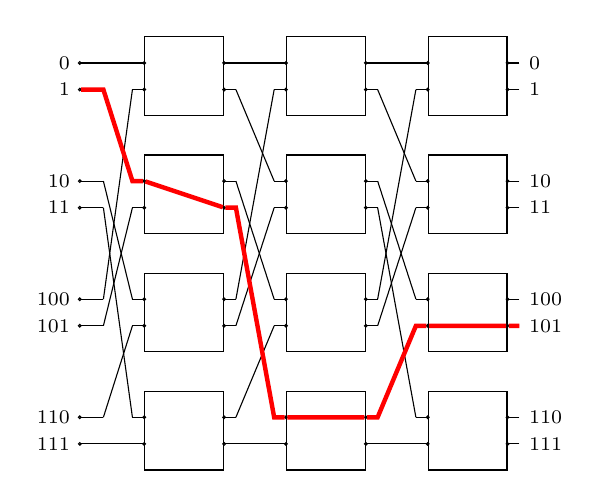
\begin{tikzpicture}
	\node[banyan omega={module label opacity=0}] {};
	\newcounter{portc}
	\setcounter{portc}{0}
	\foreach \module in {1,...,4}{
		\foreach \port in {1,...,2}{
				\stepcounter{portc}
				\pgfmathbin{\theportc-1}
				\node[left] at (r0-\module-front input-\port)
				 {\scriptsize{\pgfmathresult}}; 
				\node[right] at (r3-\module-front output-\port)
				 {\scriptsize{\pgfmathresult}};
		}
	}
	\draw[red,ultra thick]
	(r0-1-front input-2)--(r0-1-front output-2)--
	(r1-2-front input-1)--(r1-2-input-1)--
	(r1-2-output-2)--(r1-2-front output-2)--
	(r2-4-front input-1)--(r2-4-input-1)--
	(r2-4-output-1)--(r2-4-front output-1)--
	(r3-3-front input-2)-- (r3-3-input-2)--
	(r3-3-output-2)--(r3-3-front output-2);
\end{tikzpicture}
\end{codeexample}

\section{Architectures for didactic purposes}
\label{sec:dida}
To quickly draw a Clos Network  it is possible to exploit:
\begin{key}{/tikz/clos snb example}
    Option for quickly drawing a Clos Network Strictly-non-Blocking.
\end{key}
\begin{key}{/tikz/clos rear example}
    Option for quickly drawing a Clos Network Rearrangeable.
\end{key}
In this way the network is not seen in its whole complexity, but it is synthetically  depicted. An example of a Strictly-non-Blocking Clos Network drawn with this approach:
\begin{codeexample}[]
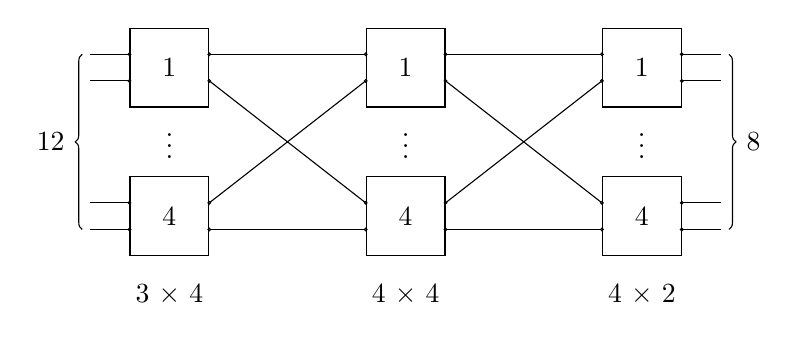
\begin{tikzpicture}[N=12,r1=4,M=8,r3=4]
    \node[clos snb example] {};
\end{tikzpicture}
\end{codeexample}

Similarly, an example of a Rearrangeable Clos Network:
\begin{codeexample}[]
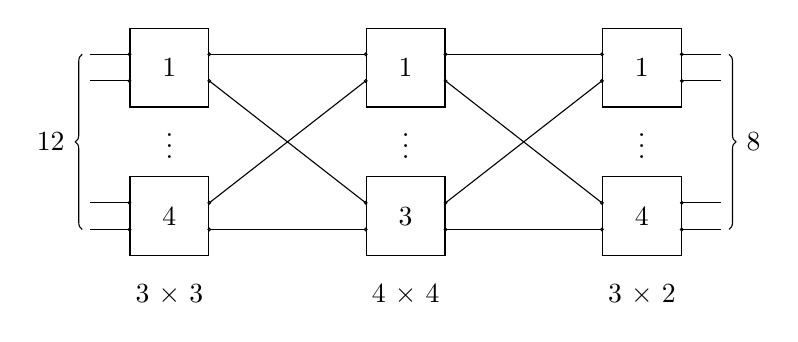
\begin{tikzpicture}[N=12,r1=4,M=8,r3=4]
    \node[clos rear example] {};
\end{tikzpicture}
\end{codeexample}

The networks drawn, automatically display the values at which the input parameters |N|, |M|, |r1| and |r3| have been set. However, to let the user to have the possibility of deploying labels rather than the input parameter values, the following option is available:

\begin{key}{/tikz/clos example with labels}
    Option for quickly drawing a Clos Network with custom labels.
\end{key}

The labels could be customized by means of:
\begin{key}{/tikz/N label=\marg{value} (default N)}
    This options sets the label representing the total number of ports in the first stage.
\end{key}

\begin{key}{/tikz/r1 label=\marg{value} (default r$_1$)}
    This options sets the label representing the number of modules in the first stage.
\end{key}

\begin{key}{/tikz/m1 label=\marg{value} (default m$_1$)}
    This options sets the label representing the number of ports per module in the first stage.
\end{key}

\begin{key}{/tikz/r2 label=\marg{value} (default r$_2$)}
    This options sets the label representing the number of modules in the second stage.
\end{key}

\begin{key}{/tikz/M label=\marg{value} (default M)}
    This options sets the label representing the total number of ports in the last stage.
\end{key}

\begin{key}{/tikz/r3 label=\marg{value} (default r$_3$)}
    This options sets the label representing the number of modules in the last stage.
\end{key}

\begin{key}{/tikz/m3 label=\marg{value} (default m$_3$)}
    This options sets the label representing the number of ports per module in the last stage.
\end{key}

An example with the default values for the labels:

\begin{codeexample}[]
%\tikzset{N=8,r1=4,M=8,r3=4} % here, setting the parameters is useless
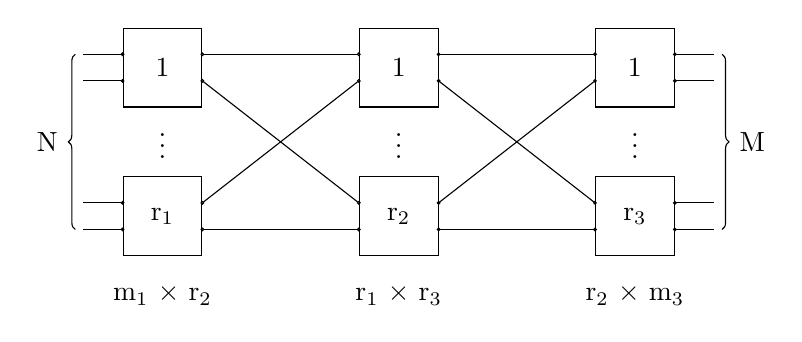
\begin{tikzpicture}
    \node[clos example with labels] {};
\end{tikzpicture}
\end{codeexample}

To have automatically all labels in math mode, use:
\begin{key}{/tikz/set math mode labels=\mchoice{true,false} (default false)}
	This option is normally disabled |set math mode labels/.default=false|; to ensure labels be set completely in math mode is sufficient set |set math mode labels=true| before the type of the network.
\end{key}

An example:
\begin{codeexample}[]
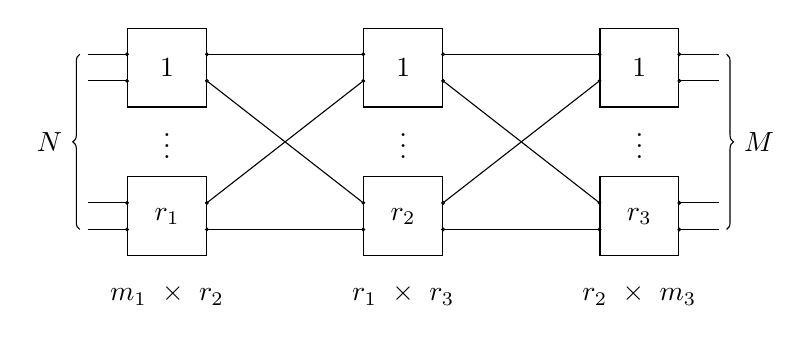
\begin{tikzpicture}[set math mode labels=true]
    \node[clos example with labels] {};
\end{tikzpicture}
\end{codeexample}

This example, instead, represents a |clos example with labels| network with custom labels introduced by means of the |\tikzset| syntax.

\begin{codeexample}[]
\tikzset{N label={p$_1$ $\times$ q$_1$},M label={p$_3$ $\times$ q$_3$}, 
r1 label=p$_1$, m1 label=q$_1$, r2 label=p$_2$,r3 label=p$_3$, m3 label=q$_3$}
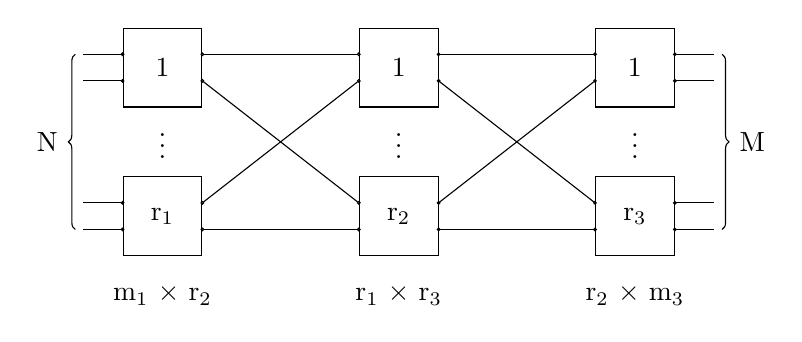
\begin{tikzpicture}
    \node[clos example with labels] {};
\end{tikzpicture}
\end{codeexample}

Notice that it does not exist an equivalent of |clos example with labels| or |clos rear example| for Benes Networks: this because Benes Networks are a particular type of Rearrangeable Clos Networks where |P|=|N|=|M| and $m1$=$m3$=$z$=2, thus |r1|=|r3|=$q=P/z$.

For example:

\begin{codeexample}[]
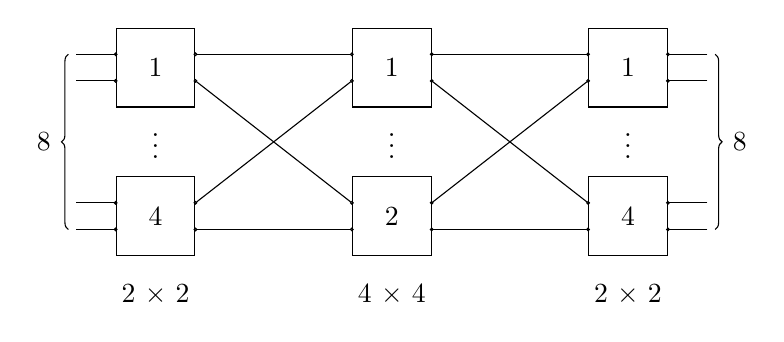
\begin{tikzpicture}[N=8,r1=4,M=8,r3=4]
    \node[clos rear example] {};
\end{tikzpicture}
\end{codeexample}

\begin{codeexample}[]
\tikzset{N label={P},M label={P}, 
r1 label=q, m1 label=z, r2 label=z,r3 label=q, m3 label=z}
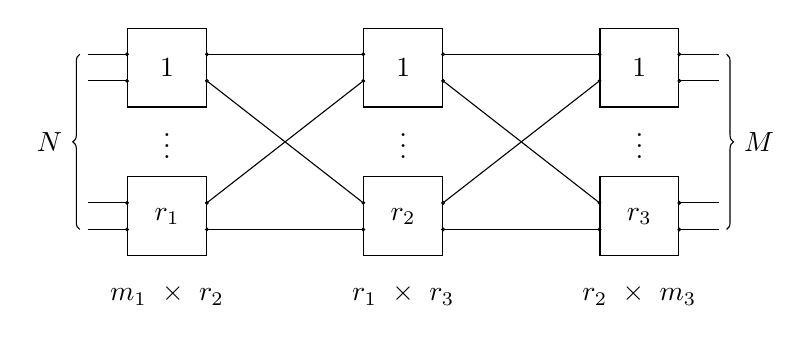
\begin{tikzpicture}
    \node[set math mode labels=true,clos example with labels] {};
\end{tikzpicture}
\end{codeexample}

\clearpage
\appendix

\section{Benes complete internal connections algorithm}
\label{sec:benesconnalg}
To explain how the connections of the |benes complete| networks are drawn, the following reference example will be considered:
\begin{center}
\scalebox{0.75}{
	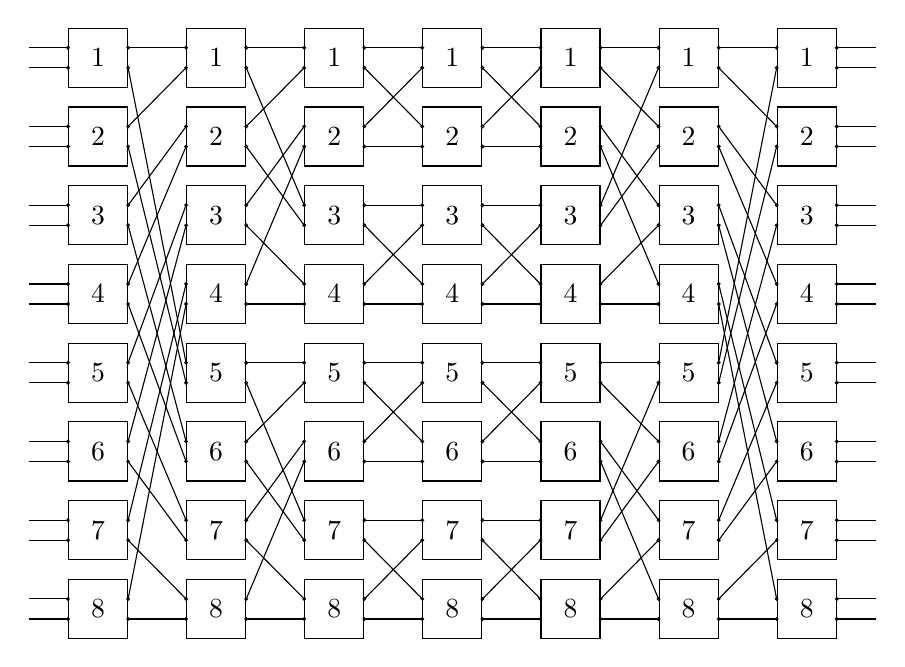
\begin{tikzpicture}[module size=0.75cm, module ysep=1, module xsep=2.5]
		\node[P=16, benes complete]{};
	\end{tikzpicture}
}
\end{center}
The network is $16\times 16$ (|P|=16), thus the number of stages $\mathcal{S}$ is:
\[\mathcal{S}=2\log_2{P}-1 \implies \mathcal{S}_{16}=7\]
Indeed:
\begin{center}
\scalebox{0.75}{
	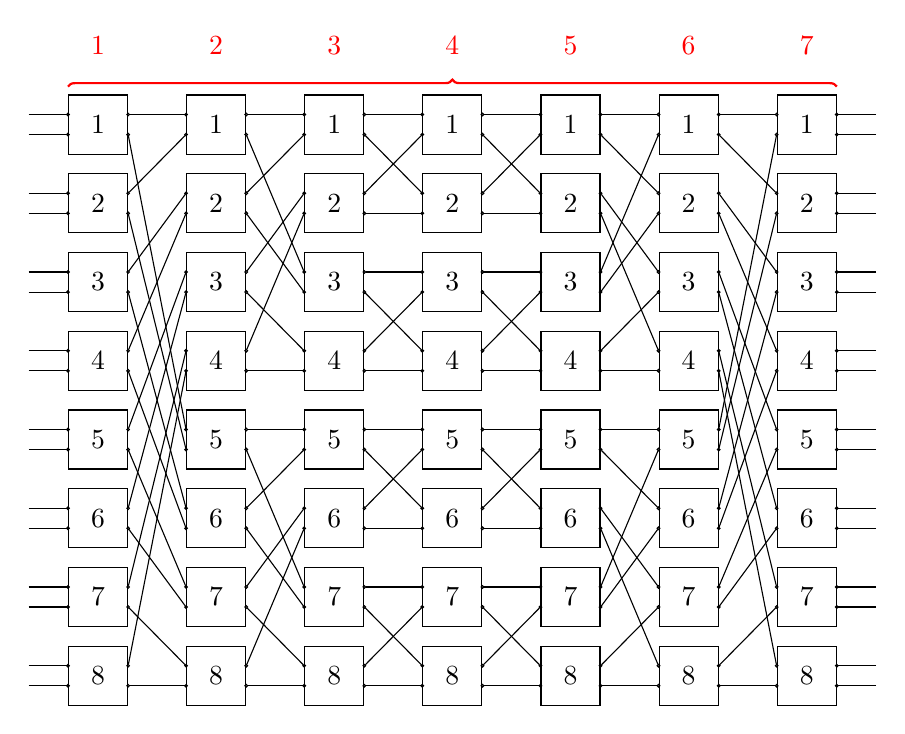
\begin{tikzpicture}[module size=0.75cm, module ysep=1, module xsep=2.5]
		\node[P=16, benes complete]{};
		\foreach \x in {1,...,7}
		\node[above of=r\x-1, red] {\x};
		\draw[red,thick,decorate,decoration={brace}]([yshift=0.1cm]r1-1.north west)--([yshift=0.1cm]r7-1.north east);
	\end{tikzpicture}
}
\end{center}
This parameter, therefore, allows to correctly draw all the modules of the network. As it will be pointed out later better, knowing |P| is also important to define the range of applicability of the algorithm among the stages. Notice the network symmetry: the connections from stage 1 to stage 4 are exactly identical to the connections from stage 7 to stage 4.  
\pagebreak

The first step is \emph{labelling} modules and ports. \saTikZ\ uses this rationale:
\begin{itemize}
\item progressive numeration for modules of the same stage;
\item progressive numeration for ports of the same module.
\end{itemize}

Thus:
\begin{center}
\scalebox{0.75}{
	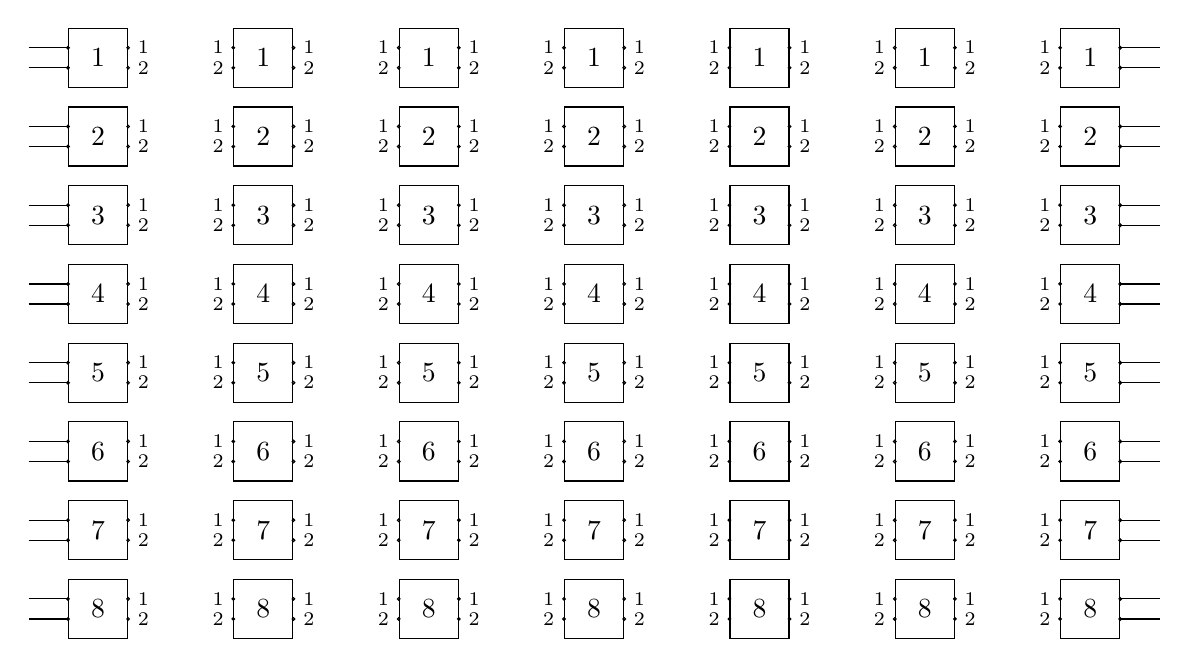
\begin{tikzpicture}[module size=0.75cm, module ysep=1, module xsep=3.5, connections disabled=true]
		\node[P=16, benes complete]{};
		\foreach \stg in {2,...,6}{
			\foreach \module in {1,...,8}{
				\node[right,font=\scriptsize] at (r\stg-\module-output-1) {1};
				\node[right,font=\scriptsize] at (r\stg-\module-output-2) {2};
				\node[left,font=\scriptsize] at (r\stg-\module-input-1) {1};
				\node[left,font=\scriptsize] at (r\stg-\module-input-2) {2};
			}
		}
		\foreach \module in {1,...,8}{
				\node[right,font=\scriptsize] at (r1-\module-output-1) {1};
				\node[right,font=\scriptsize] at (r1-\module-output-2) {2};
		}
		\foreach \module in {1,...,8}{
				\node[left,font=\scriptsize] at (r7-\module-input-1) {1};
				\node[left,font=\scriptsize] at (r7-\module-input-2) {2};
		}
	\end{tikzpicture}
}
\end{center}

Due to the network symmetry, the attention will be focused only on the left side of the network initially. On the right part of the network, things are dual.

\begin{center}
\scalebox{0.75}{
	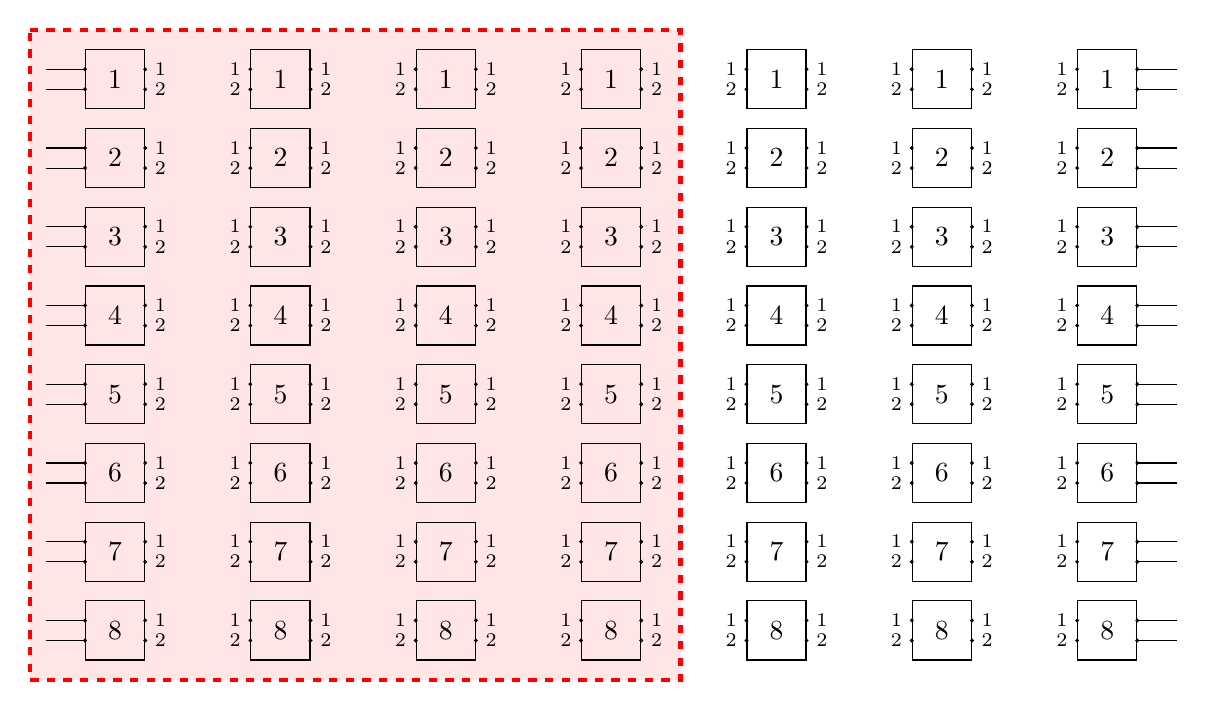
\begin{tikzpicture}[module size=0.75cm, module ysep=1, module xsep=3.5, connections disabled=true]
		\node[P=16, benes complete]{};
		\foreach \stg in {2,...,6}{
			\foreach \module in {1,...,8}{
				\node[right,font=\scriptsize] at (r\stg-\module-output-1) {1};
				\node[right,font=\scriptsize] at (r\stg-\module-output-2) {2};
				\node[left,font=\scriptsize] at (r\stg-\module-input-1) {1};
				\node[left,font=\scriptsize] at (r\stg-\module-input-2) {2};
			}
		}
		\foreach \module in {1,...,8}{
				\node[right,font=\scriptsize] at (r1-\module-output-1) {1};
				\node[right,font=\scriptsize] at (r1-\module-output-2) {2};
		}
		\foreach \module in {1,...,8}{
				\node[left,font=\scriptsize] at (r7-\module-input-1) {1};
				\node[left,font=\scriptsize] at (r7-\module-input-2) {2};
		}
		\begin{pgfonlayer}{background}
		\draw[dashed, ultra thick, red, fill=red!10]
		($(r1-1-front input-1)+(-0.2,0.5)$)--($(r4-1-output-1)+(0.5,0.5)$)--($(r4-8-output-2)-(-0.5,0.5)$)--($(r1-8-front input-2)-(0.2,0.5)$)--cycle;
		\end{pgfonlayer}
	\end{tikzpicture}
}
\end{center}
\pagebreak

Now, by drawing some connections, it is possible to find a common behaviour:

\begin{center}
\scalebox{0.75}{
	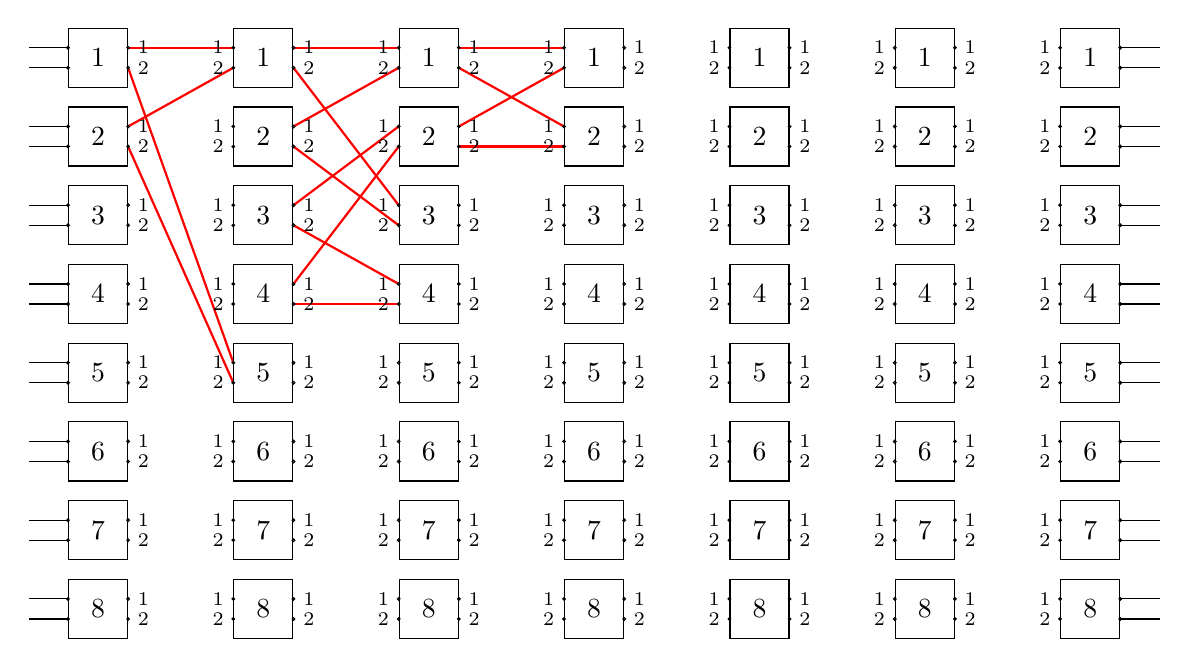
\begin{tikzpicture}[module size=0.75cm, module ysep=1, module xsep=3.5, connections disabled=true]
		\node[P=16, benes complete]{};
		\foreach \stg in {2,...,6}{
			\foreach \module in {1,...,8}{
				\node[right,font=\scriptsize] at (r\stg-\module-output-1) {1};
				\node[right,font=\scriptsize] at (r\stg-\module-output-2) {2};
				\node[left,font=\scriptsize] at (r\stg-\module-input-1) {1};
				\node[left,font=\scriptsize] at (r\stg-\module-input-2) {2};
			}
		}
		\foreach \module in {1,...,8}{
				\node[right,font=\scriptsize] at (r1-\module-output-1) {1};
				\node[right,font=\scriptsize] at (r1-\module-output-2) {2};
		}
		\foreach \module in {1,...,8}{
				\node[left,font=\scriptsize] at (r7-\module-input-1) {1};
				\node[left,font=\scriptsize] at (r7-\module-input-2) {2};
		}
		% some connections
		\begin{pgfonlayer}{background}
		% first-second stage
		\draw[thick,red](r1-1-output-1)--(r2-1-input-1);
		\draw[thick,red](r1-1-output-2)--(r2-5-input-1);
		\draw[thick,red](r1-2-output-1)--(r2-1-input-2);
		\draw[thick,red](r1-2-output-2)--(r2-5-input-2);
		% second-third stage
		\draw[thick,red](r2-1-output-1)--(r3-1-input-1);
		\draw[thick,red](r2-1-output-2)--(r3-3-input-1);
		\draw[thick,red](r2-2-output-1)--(r3-1-input-2);
		\draw[thick,red](r2-2-output-2)--(r3-3-input-2);	
		\draw[thick,red](r2-3-output-1)--(r3-2-input-1);
		\draw[thick,red](r2-3-output-2)--(r3-4-input-1);
		\draw[thick,red](r2-4-output-1)--(r3-2-input-2);
		\draw[thick,red](r2-4-output-2)--(r3-4-input-2);		
		% third-fourth stage
		\draw[thick,red](r3-1-output-1)--(r4-1-input-1);
		\draw[thick,red](r3-1-output-2)--(r4-2-input-1);
		\draw[thick,red](r3-2-output-1)--(r4-1-input-2);
		\draw[thick,red](r3-2-output-2)--(r4-2-input-2);	
		\end{pgfonlayer}		
	\end{tikzpicture}
}
\end{center}
\begin{itemize}
\item if the start module $st$ and the output port are odd (i.e. module 1, port 1), then it will be connected to  
\[\textrm{end module}=\dfrac{st+1}{2} \; , \; \textrm{port}=1 \]
\item if the start module $st$ is odd and the output port is even (i.e. module 1, port 2), then it will be connected to  
\[\textrm{end module}=\dfrac{st+1+\gamma}{2} \; , \; \textrm{port}=1 \]
\item if the start module $st$ is even and the output port is odd (i.e. module 2, port 1), then it will be connected to  
\[\textrm{end module}=\dfrac{st}{2}  \; , \; \textrm{port}=2 \]
\item if the start module $st$ and the output port are even (i.e. module 2, port 2), then it will be connected to  
\[\textrm{end module}=\dfrac{st+\gamma}{2}\; , \; \textrm{port}=2 \]
\end{itemize}

What is the term $\gamma$? It is a corrective term that depends on the starting stage. Consider, indeed, the connections of the output port 2 of module 1 in the first and in the second starting stages:
\begin{flushleft}
\texttt{r1-1-output-2} \tikz[baseline=-0.5ex]\draw[-stealth](0,0)--(0.5,0); \texttt{r2-5-input-1}\\
\texttt{r2-1-output-2} \tikz[baseline=-0.5ex]\draw[-stealth](0,0)--(0.5,0); \texttt{r3-3-input-1}
\end{flushleft}
In the first case it points to module 5 while in the second case to module 3, thus $\gamma=8$ and $\gamma=4$ in the first case and in the second case respectively. This suggest that $\gamma$ is related in some sense to the stage of the start module: in our example |P|=16, hence the relation is
\[\gamma=\dfrac{P}{2^{stage}}\]

However, following this strategy allows to draw just part of the connections:
\begin{center}
\scalebox{0.75}{
	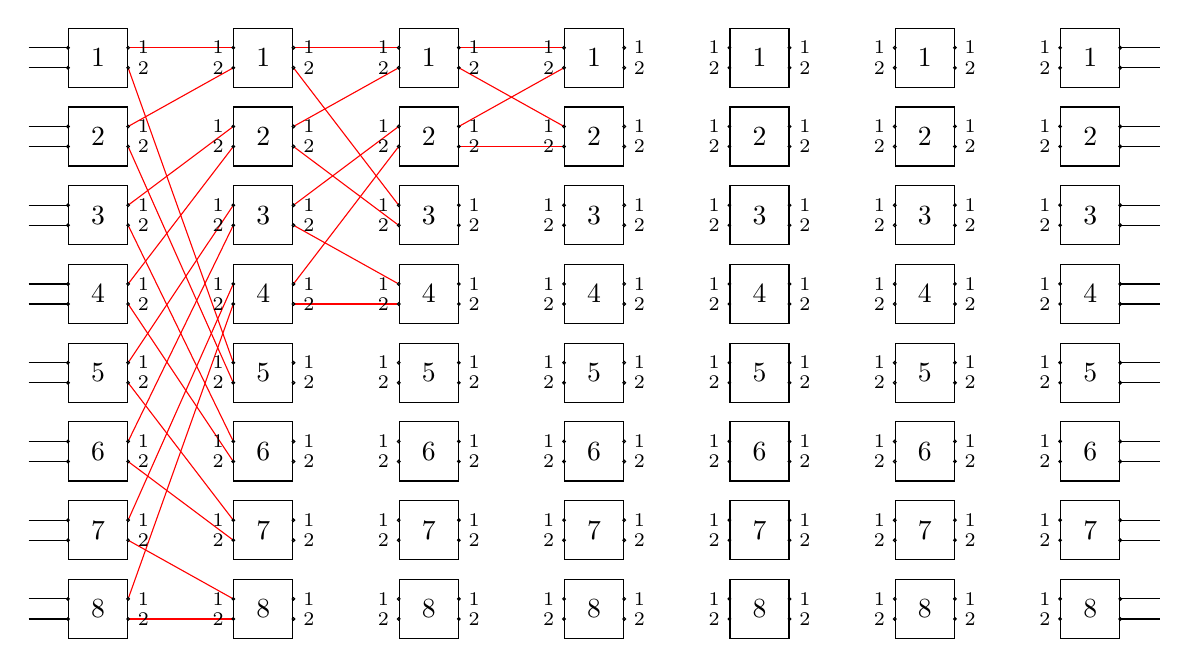
\begin{tikzpicture}[module size=0.75cm, module ysep=1, module xsep=3.5, connections disabled=true]
		\node[P=16, benes complete]{};
		\foreach \stg in {2,...,6}{
			\foreach \module in {1,...,8}{
				\node[right,font=\scriptsize] at (r\stg-\module-output-1) {1};
				\node[right,font=\scriptsize] at (r\stg-\module-output-2) {2};
				\node[left,font=\scriptsize] at (r\stg-\module-input-1) {1};
				\node[left,font=\scriptsize] at (r\stg-\module-input-2) {2};
			}
		}
		\foreach \module in {1,...,8}{
				\node[right,font=\scriptsize] at (r1-\module-output-1) {1};
				\node[right,font=\scriptsize] at (r1-\module-output-2) {2};
		}
		\foreach \module in {1,...,8}{
				\node[left,font=\scriptsize] at (r7-\module-input-1) {1};
				\node[left,font=\scriptsize] at (r7-\module-input-2) {2};
		}
		% some connections
		\begin{pgfonlayer}{background}
		\foreach \stg[evaluate=\stg as \nextstg using int(\stg+1)] in {1,...,3}{
         	\pgfmathtruncatemacro\applicationon{16/(2^\stg)}% number of modules over which the algorithm is applied
	         	\foreach \startmodule in {1,...,\applicationon}{ 
		         \pgfmathisodd{\startmodule}
			         \ifnum\pgfmathresult=1
			          % if odd
			          	\pgfmathtruncatemacro\endmodulei{int((\startmodule+1)/2)}
			          	\pgfmathtruncatemacro\endmoduleii{int(ceil(\startmodule+1+\applicationon)/2)}
			          	\draw[red](r\stg-\startmodule-output-1)--(r\nextstg-\endmodulei-input-1);
			          	\draw[red](r\stg-\startmodule-output-2)--(r\nextstg-\endmoduleii-input-1);
			          \else
			          % if even
			          	\pgfmathtruncatemacro\endmodulei{int((\startmodule)/2)}
			          	\pgfmathtruncatemacro\endmoduleii{int((\startmodule+\applicationon)/2)}
			          	\draw[red](r\stg-\startmodule-output-1)--(r\nextstg-\endmodulei-input-2);
			          	\draw[red](r\stg-\startmodule-output-2)--(r\nextstg-\endmoduleii-input-2);
			         \fi
			      }
		}	         
		\end{pgfonlayer}		
	\end{tikzpicture}
}
\end{center}
thus it is possible to claim that the algorithm has a \emph{module applicability range} that ultimately depends on the stage:
\begin{itemize}
\item in the first stage it could be applied for all modules;
\item in the second stage it could be applied for half of the modules;
\item in the third stage it could be applied just for two modules.
\end{itemize}
Since in the first stage $\gamma=8$ ($P/2^1$), in the second stage $\gamma=4$ ($P/2^2$) and in the third stage $\gamma=2$ ($P/2^3$): this means that $\gamma$ defines the \emph{module applicability range}.

Notice now, that for the second stage and the third stage, the algorithm should be simply repeated:
\begin{itemize}
\item in the second stage 2 times;
\item in the third stage 4 times.
\end{itemize}
The repetition $\psi$ depends on the stage according to the following relation:
\[\psi= 2^{stage-1}\]
Now, to draw automatically all the connections, the algorithm should know which are the starting module and ending module of the \emph{module applicability range} during the repetitions: for example, in the second stage, how to identify automatically the applicability range \texttt{1-4}, \texttt{5-8}? 

\begin{center}
\scalebox{0.75}{
	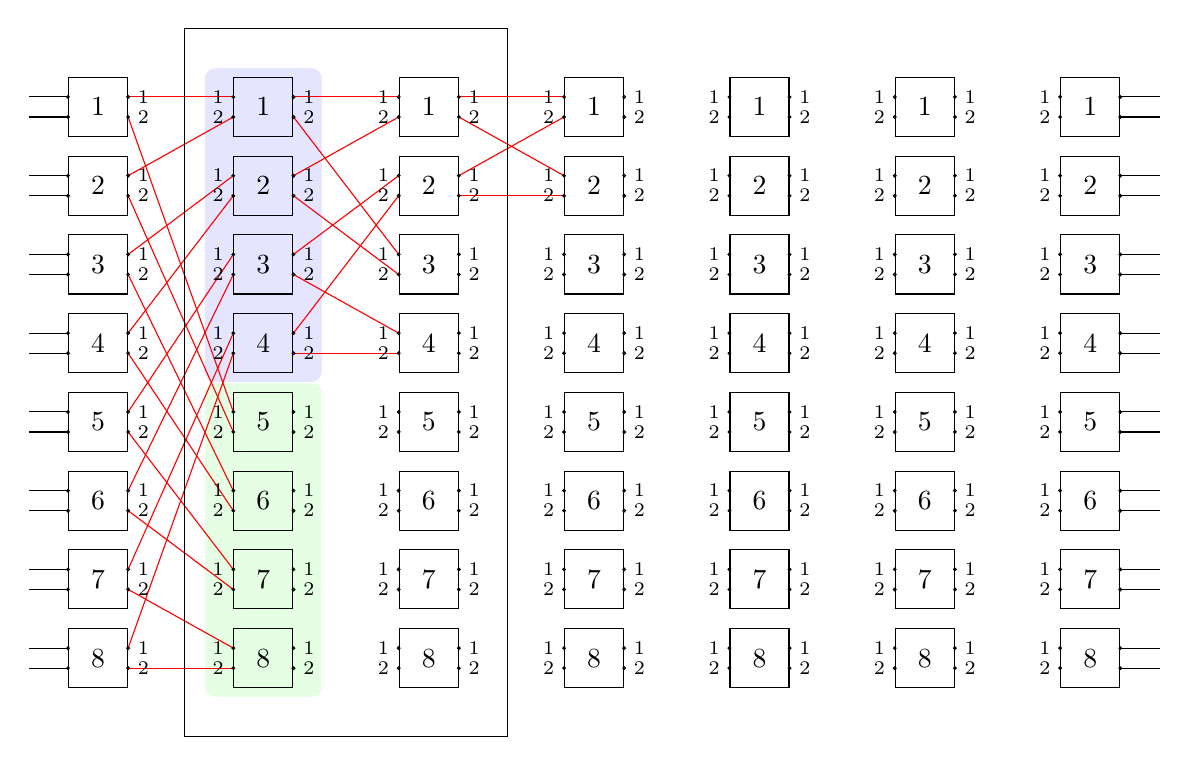
\begin{tikzpicture}[module size=0.75cm, module ysep=1, module xsep=3.5, connections disabled=true]
		\node[P=16, benes complete]{};
		\foreach \stg in {2,...,6}{
			\foreach \module in {1,...,8}{
				\node[right,font=\scriptsize] at (r\stg-\module-output-1) {1};
				\node[right,font=\scriptsize] at (r\stg-\module-output-2) {2};
				\node[left,font=\scriptsize] at (r\stg-\module-input-1) {1};
				\node[left,font=\scriptsize] at (r\stg-\module-input-2) {2};
			}
		}
		\foreach \module in {1,...,8}{
				\node[right,font=\scriptsize] at (r1-\module-output-1) {1};
				\node[right,font=\scriptsize] at (r1-\module-output-2) {2};
		}
		\foreach \module in {1,...,8}{
				\node[left,font=\scriptsize] at (r7-\module-input-1) {1};
				\node[left,font=\scriptsize] at (r7-\module-input-2) {2};
		}
		% some connections
		\begin{pgfonlayer}{background}
		\filldraw[fill=blue!10,draw=white,rounded corners]($(r2-4)-(0.75,0.5)$)rectangle ($(r2-1)+(0.75,0.5)$);
		\filldraw[fill=green!10,draw=white,rounded corners]($(r2-8)-(0.75,0.5)$)rectangle ($(r2-5)+(0.75,0.5)$);
		\foreach \stg[evaluate=\stg as \nextstg using int(\stg+1)] in {1,...,3}{
         	\pgfmathtruncatemacro\applicationon{16/(2^\stg)}% number of modules over which the algorithm is applied
	         	\foreach \startmodule in {1,...,\applicationon}{ 
		         \pgfmathisodd{\startmodule}
			         \ifnum\pgfmathresult=1
			          % if odd
			          	\pgfmathtruncatemacro\endmodulei{int((\startmodule+1)/2)}
			          	\pgfmathtruncatemacro\endmoduleii{int(ceil(\startmodule+1+\applicationon)/2)}
			          	\draw[red](r\stg-\startmodule-output-1)--(r\nextstg-\endmodulei-input-1);
			          	\draw[red](r\stg-\startmodule-output-2)--(r\nextstg-\endmoduleii-input-1);
			          \else
			          % if even
			          	\pgfmathtruncatemacro\endmodulei{int((\startmodule)/2)}
			          	\pgfmathtruncatemacro\endmoduleii{int((\startmodule+\applicationon)/2)}
			          	\draw[red](r\stg-\startmodule-output-1)--(r\nextstg-\endmodulei-input-2);
			          	\draw[red](r\stg-\startmodule-output-2)--(r\nextstg-\endmoduleii-input-2);
			         \fi
			      }
		}
		
		\draw($(r2-8)-(1,1)$)rectangle ($(r3-1)+(1,1)$);
		\end{pgfonlayer}		
	\end{tikzpicture}
}
\end{center}

They could be defined as:
\begin{itemize}
\item starting module: $st_m=1+(\psi-1)\cdot\gamma $;
\item ending module: $end_m=(st_m+\gamma)-1$.
\end{itemize}
Indeed, for the second stage we have that $\gamma=4$ and $\psi=2\implies \{1,\, 2\}$, hence there are two starting and ending modules:
\begin{itemize}
\item starting modules: $st_{m_1}=1+(1-1)\cdot 4=1$ and $st_{m_2}=1+(2-1)\cdot 4=5$;
\item ending modules:  $end_{m_1}=(1+4)-1=4$ and $end_{m_2}=(5+4)-1=8$.
\end{itemize}
Unfortunately, the knowledge of the starting and ending modules of each stage is not sufficient to reach the goal: the reason is that the algorithm works and draws the connections in a correct manner when the module labels start with 1. However, during the repetitions the new starting module labels are different, thus the computation of the end connection point fails. This difference should be compensated with \emph{shifts} of the ending modules that depend on the level of repetition. The rules are:
\begin{itemize}
\item if $\psi=1$ (the algorithm works for all modules of the stage), then the ending module of the connection is computed as:
\begin{itemize}
\item if the start module $st$ and the output port are odd (i.e. module 1, port 1), then it will be connected to  
\[\textrm{end module}=\dfrac{st+1}{2} \; , \; \textrm{port}=1 \]
\item if the start module $st$ is odd and the output port is even (i.e. module 1, port 2), then it will be connected to  
\[\textrm{end module}=\dfrac{st+1+\gamma}{2}\; , \; \textrm{port}=1 \]
\item if the start module $st$ is even and the output port is odd (i.e. module 2, port 1), then it will be connected to  
\[\textrm{end module}=\dfrac{st}{2}  \; , \; \textrm{port}=2 \]
\item if the start module $st$ and the output port are even (i.e. module 2, port 2), then it will be connected to  
\[\textrm{end module}=\dfrac{st+\gamma}{2}\; , \; \textrm{port}=2 \]
\end{itemize}
\item if $\psi=2$ (the algorithm should be repeated twice), then the ending module of the connection is computed as
\begin{itemize}
\item if the start module $st$ and the output port are odd (i.e. module 1, port 1), then it will be connected to  
\[\textrm{end module}=\dfrac{st+1}{2}+\dfrac{\gamma}{2} \; , \; \textrm{port}=1 \]
\item if the start module $st$ is odd and the output port is even (i.e. module 1, port 2), then it will be connected to  
\[\textrm{end module}=\dfrac{st+1+\gamma}{2}+\dfrac{\gamma}{2}\; , \; \textrm{port}=1 \]
\item if the start module $st$ is even and the output port is odd (i.e. module 2, port 1), then it will be connected to  
\[\textrm{end module}=\dfrac{st}{2}+\dfrac{\gamma}{2}  \; , \; \textrm{port}=2 \]
\item if the start module $st$ and the output port are even (i.e. module 2, port 2), then it will be connected to  
\[\textrm{end module}=\dfrac{st+\gamma}{2}+\dfrac{\gamma}{2}\; , \; \textrm{port}=2 \]
\end{itemize}
\item if $\psi>2\implies t=3,\ldots, \psi$ (the algorithm should be repeated more than twice), then the ending module of the connection is computed as:
\begin{itemize}
\item if the start module $st$ and the output port are odd (i.e. module 1, port 1), then it will be connected to  
\[\textrm{end module}=\dfrac{st+1}{2}+\left(\dfrac{\gamma}{2}\cdot (t-2)\right) \; , \; \textrm{port}=1 \]
\item if the start module $st$ is odd and the output port is even (i.e. module 1, port 2), then it will be connected to  
\[\textrm{end module}=\dfrac{st+1+\gamma}{2}+\dfrac{\gamma}{2}+\left(\dfrac{\gamma}{2}\cdot (t-2)\right)\; , \; \textrm{port}=1 \]
\item if the start module $st$ is even and the output port is odd (i.e. module 2, port 1), then it will be connected to  
\[\textrm{end module}=\dfrac{st}{2}+\left(\dfrac{\gamma}{2}\cdot (t-2)\right)\; , \; \textrm{port}=2 \]
\item if the start module $st$ and the output port are even (i.e. module 2, port 2), then it will be connected to  
\[\textrm{end module}=\dfrac{st+\gamma}{2}+\dfrac{\gamma}{2}+\left(\dfrac{\gamma}{2}\cdot (t-2)\right)\; , \; \textrm{port}=2 \]
\end{itemize}
\end{itemize}
Unfortunately, the rule $\psi>2$ when it is applied to the intermediate stages 
\[I_1=\lfloor\mathcal{S}\div 2\rfloor \hspace*{1cm} I_2=\mathcal{S}-(I_1-1)\]
does not work; this implies that:
\begin{itemize}
\item on the left side of the network the applicability of the algorithm is from the starting stage 1 up to the starting stage $I_1-1$ (in the example |P|=16: from the starting stage 1 up to the starting stage 2);
\item on the right side of the network the applicability of the algorithm is from the starting stage $\mathcal{S}$ up to the starting stage $I_2-1$ (in the example |P|=16: from the starting stage 7 up to the starting stage 6);
\item for the intermediate starting stages $I_1$ and  $I_2$ (in the example |P|=16: the stages 3 and 5) another rule should be used:
\begin{itemize}
\item if the start module $st$ and the output port are odd (i.e. module 1, port 1), then it will be connected to  
\[\textrm{end module}=st\; , \; \textrm{port}=1 \]
\item if the start module $st$ is odd and the output port is even (i.e. module 1, port 2), then it will be connected to  
\[\textrm{end module}=st+1\; , \; \textrm{port}=1 \]
\item if the start module $st$ is even and the output port is odd (i.e. module 2, port 1), then it will be connected to  
\[\textrm{end module}=st-1  \; , \; \textrm{port}=2 \]
\item if the start module $st$ and the output port are even (i.e. module 2, port 2), then it will be connected to  
\[\textrm{end module}=st\; , \; \textrm{port}=2 \]
\end{itemize}
\end{itemize}

To summarize, the algorithm to \textbf{d}raw \textbf{B}enes \textbf{n}etwork \textbf{c}onnections (dBnc) is reported in~\ref{algo_dBnc}: for the rules, please refer to the afore-mentioned description.

\begin{algorithm}
compute $\mathcal{S}=2\log_2{P}-1$\;
compute $I_1=\lfloor\mathcal{S}\div 2\rfloor$\;
compute $I_2=\mathcal{S}-(I_1-1)$\;
\emph{from left to right}\;
\For{$stg\leftarrow 1$ \KwTo $(I_1-1)$}{
	compute $\gamma=P\div 2^{stg}$\;
	compute $\psi=2^{stg-1}$\;
	\For{$t\leftarrow 1$ \KwTo $\psi$}{
		compute starting point $x=1+((t-1)\cdot\gamma)$\;
		compute ending point $y=(x+\gamma)-1$\;
		\ForEach{$\textrm{ start module } s \textrm{ in set } (x,y)$}{
			\uIf{$t==1$}{
				\uIf{$s$ is odd}{
					use rules $\psi=1$ for starting module odd\;
				}
				\Else{
					use rules $\psi=1$ for starting module even\;
				}
			}
			\uIf{$t==2$}{
				\uIf{$s$ is odd}{
					use rules $\psi=2$ for starting module odd\;
				}
				\Else{
					use rules $\psi=2$ for starting module even\;
				}
			}
			\uIf{$t>2$}{
				\uIf{$s$ is odd}{
					use rules $\psi>2$ for starting module odd\;
				}
				\Else{
					use rules $\psi>2$ for starting module even\;
				}
			}
		}
	}
}
\emph{from right to left}\;
\For{$stg\leftarrow \mathcal{S}$ \KwTo $(I_2-1)$}{
	repeat in dual mode $\textbf{6}-\textbf{32}$\;
}
\emph{complete with intermediate stages}\;
\ForEach{$stg$ in set $(I_1,\, I_2)$}{
	use rules for intermediate stages\;
}
\caption{\textbf{d}raw \textbf{B}enes \textbf{n}etwork \textbf{c}onnections (dBnc)}\label{algo_dBnc}
\end{algorithm}


% * * * * * * * * * * * * * * * * * * * * * * * * * * 
% belongs to \usepackage{makeindex}
\printindex
\end{document}
